%
% chapter.tex -- Krümmung
%
% (c) 2025 Prof Dr Andreas Müller
%
\chapter{Krümmung
\label{chapter:kruemmung}}
\kopflinks{Krümmung}

\noindent
In Abbildung~\ref{buch:kruemmung:fig:exzess}
%
% fig-exzess.tex
%
% (c) 2025 Prof Dr Andreas Müller
%
\begin{figure}
\centering
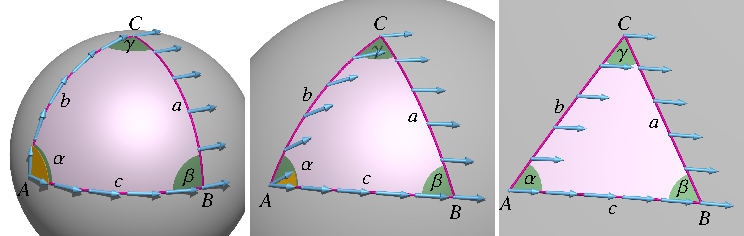
\includegraphics{chapters/110-kruemmung/images/exzess.pdf}
\caption{Der Paralleltransport eines Tangentialvektors um ein 
sphärisches Dreieck führt wegen der Krümmung der Kugeloberfläche
zu einer Drehung des Vektors um den orangen Winkel beim Punkt $A$.
Für kleine Dreiecke bzw.~grosse Kugelradien nähert sich das
Dreieck einem ebenen Dreieck an und die Drehung wird sehr klein.
\label{buch:kruemmung:fig:exzess}}
\end{figure}

%
% fig-drehung.tex
%
% (c) 2025 Prof Dr Andreas Müller
%
\begin{figure}
\centering
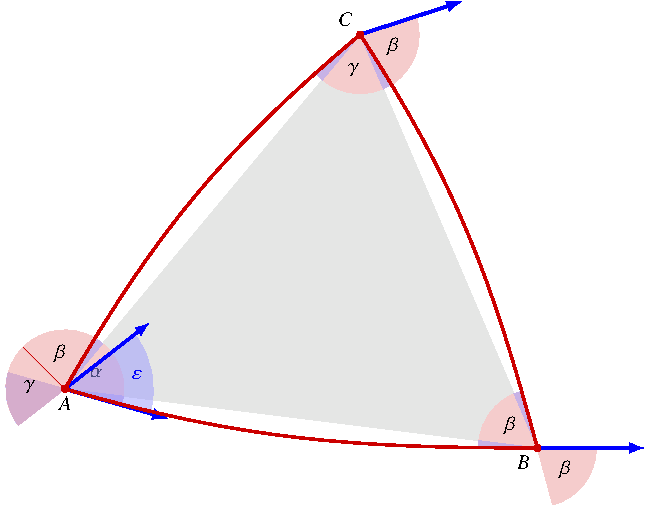
\includegraphics{chapters/110-kruemmung/images/drehung.pdf}
\caption{Die Drehung eines Vektors beim Paralleltransport eines
Tangentialvektors ausgehend vom Punkt $A$ entlang der Seiten eines
sphärischen Dreiecks entlang der Seiten des Dreiecks resultiert
in einer Drehung um den blauen Winkel.
Er ist gleich gross wie die Summe der in jeder Ecke eingezeichneten
kleinen blauen Winkel, die anzeigen, wieviel grösser die Winkel
des sphärischen Dreiecks sind als die des ebenen Dreiecks
$\triangle ABC$.
Ihre Summe heisst daher der sphärische Exzess
$\varepsilon = \alpha+\beta+\gamma-\pi$.
\label{buch:kruemmung:fig:drehung}}
\end{figure}

sind gleichseitige sphärische Dreiecke zu unterschiedlichen
Kugelradien dargestellt.
Die Seiten $a=b=c$ sind gleich, ebenso die Winkel $\alpha=\beta=\gamma$.
Das Dreieck ganz rechts ist im Vergleich zum Kugelradius so klein,
dass die Krümmung kaum mehr sichtbar ist.
Nach dem Seitenkosinussatz
\[
\cos c = \cos a\cos b + \sin a \sin b \cos\alpha
\]
der sphärischen Trigonometrie folgt für das gleichseitige Dreieck
\begin{align*}
\cos a-\cos^2a
&=
\sin^2 a \cos\alpha
=
(1-\cos^2 a)\cos\alpha
\\
\cos a(1-\cos a)
&=
(1+\cos a)(1-\cos a)\cos\alpha
\intertext{und nach Division durch $1-\cos a$}
\frac{ \cos a }{ 1+\cos a }
&=
\cos\alpha.
\end{align*}
Im Grenzwert $a\to 0$ strebt $\cos a$ gegen 1.
Der Grenzwert für den Winkel $\alpha$ ergibt sich daher aus
$\cos\alpha=\frac12$ als $\alpha=60^\circ$.

Der Transport des Tangentialvektors entlang der Seite $AB$ eines
beliebigen sphärischen Dreiecks wie in
Abbildung~\ref{buch:kruemmung:fig:drehung}
liefert den Tangentialvektor an $AB$ im Punkt $B$.
Dieser schliesst mit der Seite $BC$ den Winkel $\beta$ ein.
Der Paralleltransport dieses Vektors ergibt einen Vektor im Punkt $C$,
der mit der Seite $CA$ einen Winkel $\beta+\gamma$ einschliesst.
Durch Paralleltransport zum Punkt $A$ ergibt sich eine Drehung um
insgesamt $\varepsilon= \alpha+\beta+\gamma -\pi$.
Die Grösse $\varepsilon$ ist bekannt als der {\em sphärische Exzess}
\index{Exzess, spharisch@Exzess, sphärisch}%
\index{spharischer Exzess@sphärischer Exzess}%
Bei einem ebenen Dreieck verschwindet der sphärische Exzess,
beim Paralleltransport eines Vektors ist keine Drehung feststellbar.

Beim gleichseitigen sphärischen Dreieck von
Abbildung~\ref{buch:kruemmung:fig:exzess}
sind alle Winkel gleich gross, der sphärische Exzess und damit die
Drehung des Tangentialvektors ist daher $\varepsilon=3\alpha-\pi$. 
Er erreicht für ein Dreieck mit drei rechten Winkeln und drei
Seiten der Längen $\frac{\pi}2$ den Wert $\frac{\pi}2$.

Der sphärische Exzess eines sphärischen Dreiecks ist auch ein Mass für
den Flächeninhalt $\Delta F = (\alpha+\beta+\gamma-\pi)R^2$.
Je grösser der Flächeninhalt in Relation zur Oberfläche der Kugel,
desto grösser die Drehung beim Paralleltransport eines Vektors um
ein Dreieck.
Oder je grösser der Drehwinkel, desto grösser die Krümmung $1/R^2$
der Kugeloberfläche.
Die Krümmung einer Fläche kann also verallgemeinert werden als
der Grenzwert des Verhältnisses des Drehwinkels eines Vektors um einen
geschlossenen polygonalen Weg zum Flächeninhalt des Polygons für
sehr kleine Polygone.

In Abschnitt~\ref{buch:kruemmung:section:riemann} dieses Kapitels
wird der riemannsche Krümmungstensor als eine lineare Abbildung,
die aus einem 2-Vektor eine Drehmatrix berechnet.
Zur Charakterisierung kann man aber auch nur einzelne Invarianten
der Drehmatrix verwenden.
Zum Beispiel lässt sich der Drehwinkel aus der Spur der Drehmatrix
berechnen.
Die Spur des riemannschen Krümmungstensors wird daher in 
Abschnitt~\ref{buch:kruemmung:section:riemann} als der Ricci-Tensor
eingeführt.
Aus dem Ricci-Tensor lassen sich die Einsteinschen Feldgleichungen
konstruieren, wie Abschnitt~\ref{buch:kruemmung:section:gravitation}
gezeigt wird.
Damit werden dann Aussagen über schwarze Löcher
(Abschnitt~\ref{buch:kruemmung:section:schwarzesloch})
und die Geschichte des Universums
(Abschnitt~\ref{buch:kruemmung:section:friedmann})
ableiten.

%
% Der riemannsche Krümmungstensor
%
\section{Berechnung der Krümmung
\label{buch:kruemmung:section:riemann}}
\kopfrechts{Berechnung der Krümmung}
Das eingangs am Beispiel des Paralleltransports entlang eines
Dreiecksweges auf einer Kugeloberfläche illustrierte Phänomen
der Drehung eines paralleltransportierten Vektors soll jetzt
als Ausgangspunkt der Definition eines Krümmungsmasses sein.
Im Geiste der früheren Kapitel muss die Krümmung als eine 2-Form
beschrieben werden können, da die Krümmung offenbar durch Bewegung
entlang des Randes eines Flächenstücks erkennbar wird.
Allerdings können die Werte nicht nur skalare Werte sein, da
sich die Drehung eines Vektors nur mit Hilfe einer Matrix
beschreiben lässt.
Wir erwarten daher einen Tensor vierter Stufe.
Dieser Tensor ist der riemannsche Krümmungstensor.

%
% Der riemannsche Krümmungstensor
%
\subsection{Der riemannsche Krümmungstensor}
Das Einführungsbeispiel der Winkeldrehung eines paralleltransportieren
Vektors motiviert die Definition der Krümmung als die Abbildung 
der Tangentialvektoren beim Paralleltransport.
Ein Koordinatenparallelgramm mit den Ecken
\begin{center}
\begin{tikzpicture}[>=latex,thick]
\begin{scope}[xshift=-6cm,yshift=-0cm]
\node at (0,0) {$\displaystyle
\begin{aligned}
A &= x,\\
B &= x+\vec{h},\\
C &= x+\vec{h}+\vec{k}\\
\text{und}\quad
D &= x+\vec{k}
\end{aligned}$};
\end{scope}
\begin{scope}
\coordinate (A) at (-1.5,-1);
\coordinate (B) at (1.0,-0.5);
\coordinate (C) at (1.5,1);
\coordinate (D) at (-1.0,0.5);
\fill[color=gray!20] (A) -- (B) -- (C) -- (D) -- cycle;
\node at ($0.25*(A)+0.25*(B)+0.25*(C)+0.25*(D)$) {$\vec{h}\wedge\vec{k}$};
\draw[->] (A) -- (B);
\draw[->] (B) -- (C);
\draw[->] (C) -- (D);
\draw[->] (D) -- (A);
\fill (A) circle[radius=0.05];
\fill (B) circle[radius=0.05];
\fill (C) circle[radius=0.05];
\fill (D) circle[radius=0.05];
\node at (A) [below left] {$A$};
\node at (B) [below right] {$B$};
\node at (C) [above right] {$C$};
\node at (D) [above left] {$D$};
\node at ($0.5*(A)+0.5*(B)$) [below] {$\vec{h}$};
\node at ($0.5*(A)+0.5*(D)$) [left] {$-\vec{k}$};
\node at ($0.5*(B)+0.5*(C)$) [right] {$\vec{k}$};
\node at ($0.5*(D)+0.5*(C)$) [above] {$-\vec{h}$};
\end{scope}
\end{tikzpicture}
\end{center}
hat als Rand einen geschlossen Pfad, entlang dem ein Vektor parallel
transportiert werden soll.
Ein Vektor $A$ mit den Komponenten $a^i$ wird beim Transport entlang
des Weges linear abgebildet auf einen Vektor
$R(\vec{h}\wedge\vec{k})\cdot A$ abgebildet, der in linearer Näherung
nur vom 2-Vektor $\vec{h}\wedge\vec{k}$ und vom Vektor $A$ abhängt.
Der {\em riemannsche Krümmungstensor} ist daher die lineare Abbildung
\index{riemannscher Krummungstensor@riemannscher Krümmungstensor}%
$R(\vec{h}\wedge\vec{k})$.

%
% Tangentialvektoren der Drehgruppen
%
\subsubsection{Tangentialvektoren der Drehgruppen}
Der Krümmungstensor hängt antisymmetrisch von den Komponenten von
$\vec{h}$ und $\vec{k}$ ab und liefert eine Matrix, die von einer
Drehung herrührt.
Sei also $D(t)\in\operatorname{SO}(n)$ ein Weg in der Gruppe
der $n$-dimensionalen Drehmatrizen, die beim Parameterwert $t=0$
durch die Einheitsmatrix $I\in \operatorname{SO}(n)$ geht.
Er erfüllt
\begin{align*}
D(t)^tD(t) &= I
&&\text{und}&
\det D(t) &= 1.
\intertext{Die Ableitung nach $t$ an der Stelle $t=0$ ist}
\bigl(
\dot{D}(t)^tD(t)
+
D(t)^t\dot{D}^t
\bigr)\Bigl|_{t=0}
&=
0
&&\text{und}&
\operatorname{Spur}\dot{D}(0)
&=
0.
\end{align*}
Aus der linken Gleichung wird mit $D(0)=I$ die Bedingung
\[
\dot{D}(0) + \dot{D}(0)^t
\qquad\Rightarrow\qquad
\dot{D}(0)^t
=
-\dot{D}(0).
\]
Die Tangentialvektoren an die Drehgruppe sind als antisymmetrische
Matrizen mit verschwindender Spur.

\begin{beispiel}
Die Matrizen in der zweidimensionalen Drehmatrix sind
\[
D(t)
=
\begin{pmatrix}
\cos kt &          - \sin kt\\
\sin kt & \phantom{-}\cos kt
\end{pmatrix}
\]
mit der Ableitung
\[
\dot{D}(0)
=
\begin{pmatrix}
0 & -k\\
k &\phantom{-}0
\end{pmatrix}.
\qedhere
\]
\end{beispiel}

Die oben durchgeführten Rechnungen gelten nur in $\operatorname{SO}(n)$,
die mit dem Standardskalarprodukt definiert wird.
Auf einer beliebigen riemannschen Mannigfaltigkeit sind Drehmatrizen $D$
durch die Eigenschaft gegeben, dass
\[
D^t(t)GD(t)
=
G
\]
gilt.
Durch Ableitung nach $t$ an der Stelle $t=0$ folgt
\[
\dot{D}(0)^tG + G\dot{D}(0)
=
0
\qquad\Rightarrow\qquad
G\dot{D}(0)
=
-\dot{D}(0)^tG.
\]
Schreibt man die Komponenten von $\dot{D}(0)$ als $D^i\mathstrut_l$,
dann bedeutet dies
\[
g_{uv}D^{v}\mathstrut_l
=
-
\sum_{v}
D^{u}\mathstrut_v
g_{vl}
\]
Zieht man den oberen Index von $D^u\mathstrut_v$ mit herunter,
entsteht ein symmetrischer Tensor
\[
D_{uv}
=
g_{ui} D^i\mathstrut_v
\qquad\Rightarrow\qquad
D_{uv}
=
-D_{vu}.
\]

%
% Symmetrien des Krümmungstensors
%
\subsubsection{Symmetrien des Krümmungstensors}
Der Krümmungstensor $R(\vec{h}\wedge\vec{k})$ hat als Wert eine Matrix,
deren Komponenten wir mit $R^i\mathstrut_l$ bezeichnen können.
Sie hängt antisymmetrisch von den Komponenten der beiden Vektoren
$\vec{h}\wedge\vec{k}$ ab.
In Komponenten ausgedrückt ist also
\[
R^i\mathstrut_l(\vec{h}\wedge\vec{k})
=
R^i\mathstrut_{luv} h^uk^v,
\]
wobei wie üblich nach der einsteinschen Summationskonvention über $u$
$v$ summiert werden muss.
Falls der metrische Tensor die Einheitsmatrix ist, muss $R^i\mathstrut_l$
antisymmetrisch sein, doch dies ist keine Eigenschaft, die allgemein
kovariant definiert ist.
Aus den Resultaten des letzten Abschnitts folgt aber, dass nach
Herunterziehen des oberen Index mithilfe von $g_{uv}$ eine
antismmetrische Matrix entsteht.
Für beliebige Vektoren $\vec{h}$ und $\vec{v}$ muss daher
$g_{li}R^i\mathstrut_l(\vec{h}\wedge\vec{k})=R_{il}(\vec{h}\wedge\vec{k})$
ein antisymmetrischer Tensor zweiter Stufe sein.
In Komponenten muss für beliebige Indizes $u$ und $v$ muss
$R_{jluv}=g_{ji}R^i\mathstrut_{luv}$ antisymmetrisch in den
Indizes $j$ und $l$ sein.

%
% Kovariante bleitung und Krümmungstensor
%
\subsubsection{Kovariante Ableitung und Krümmungstensor}
Wir berechnen jetzt den Paralleltransport des Vektors mit den
Komponenten $a^i$ entlang der Kantenpfade $ABC$ und $ADC$ 
des von $\vec{h}$ und $\vec{k}$ aufgespannten Parallelogramms.
Der Transport von $A$ nach $B$ ändert den Vektor um die Komponenten
\[
-\Gamma^l_{uv} a^u h^v 
\]
Der neue Vektor muss jetzt um den Vektor $\vec{k}$ transportiert
werden, der transportierte Vektor ist
\[
b^l
=
a^l-\Gamma^l_{uv} a^u h^v.
\]
Dies ergibt
\begin{align*}
\biggl(
\frac{\partial b^s}{\partial x^m}
+
\Gamma^s_{nm} b^n
\biggr)
k^m
&=
\biggl(
\frac{\partial \Gamma^s_{uv}}{\partial x^m}
a^u
h^v
-
\Gamma^s_{nm}
a^n
+
\Gamma^s_{nm} \Gamma^n_{uv}
a^u
h^v
\biggr)
k^m
\\
&=
\biggl(
\frac{\partial \Gamma^s_{uv}}{\partial x^m}
+
\Gamma^s_{nm}\Gamma^n_{uv}
\biggr)
a^u
h^v k^m
-
\Gamma^s_{nm}a^nk^m.
\end{align*}
Vertauschung von $v$ und $m$ führt auf den entsprechenden
Ausdruck für den Weg $ADC$.
Die Differenz ist der gesucht Krümmungstensor
\begin{align}
R^s\mathstrut_{uvm}
&=
\frac{\partial\Gamma^s_{uv}}{\partial x^m}
-
\frac{\partial\Gamma^s_{um}}{\partial x^v}
-
\Gamma^s_{nm}\Gamma^n_{uv}
+
\Gamma^s_{nv}\Gamma^n_{um}
\label{buch:kruemmung:kruemmung:eqn:Rm}
\end{align}
Dies sind die Komponenten des riemannschen Krümmungstensors.
Durch herunterziehen des ersten Index erhält man die Komponenten
\begin{equation}
R_{ruvm}
=
g_{rs}
\biggl(
\frac{\partial\Gamma^s_{uv}}{\partial x^m}
-
\frac{\partial\Gamma^s_{um}}{\partial x^v}
-
\Gamma^s_{nm}\Gamma^n_{uv}
+
\Gamma^s_{nv}\Gamma^n_{um}
\biggr)
\label{buch:kruemmung:kruemmung:eqn:Rmkovariant}
\end{equation}
des kovarianten riemannschen Tensors.
Er ist antisymmetrisch in den ersten zwei und den letzten zwei
Indizes.

\begin{beispiel}
Der riemannsche Krümmungstensor für die Ebene in Polarkoordinaten.
\\[5pt]
In Polarkoordinaten $(r,\vartheta)$ wird die euklidische Metrik
durch die Koeffizienten
\[
g_{11} = 1,\quad
g_{22} = r^2,\qquad
g
=
\begin{pmatrix}
1&0\\
0&r^2
\end{pmatrix},
\quad
g^{-1}
=
\begin{pmatrix}
1&0\\
0&r^{-2}
\end{pmatrix},
\]
gegeben.
Daraus kann man die Christoffel-Symbole erster Art
\begin{align*}
\Gamma_{1,11}                 & =  0 &
\Gamma_{1,12} = \Gamma_{1,21} & =  0 &
\Gamma_{1,22}                 & = -r
\\
\Gamma_{2,11}                 & = 0 &
\Gamma_{2,12} = \Gamma_{2,21} & = r &
\Gamma_{2,22}                 & = 0
\intertext{und zweiter Art}
\Gamma^1_{11}                 & = 0  &
\Gamma^1_{12} = \Gamma^1_{21} & =  0 &
\Gamma^1_{22}                 & = -r
\\
\Gamma^2_{11}                 & = 0  &
\Gamma^2_{12} = \Gamma^2_{21} & = \frac{1}{r} &
\Gamma^2_{22}                 & = 0
\end{align*}
berechnen.
Verwendet man diese Koeffizienten, um den riemannschen Krümmungstensor
zu berechnen, erhält man $0$ für alle Komponenten.
\end{beispiel}

\begin{beispiel}
\label{buch:kruemmung:kruemmung:bsp:kugel}
Der riemannsche Krümmungstensor für die Kugeloberfläche.
\\[5pt]
Auf der Oberfläche einer Einheitskugel hat die Metrik in Kugelkoordinaten
$(\vartheta,\varphi)$
die metrischen Koeffizienten
\[
g_{11} = 1,\quad
g_{22} = \sin^2\vartheta
\qquad
\Rightarrow
\qquad
g
=
\begin{pmatrix}
1&0\\0&\sin^2\vartheta
\end{pmatrix},
\quad
g^{-1}
=
\begin{pmatrix}
1&0\\0&\frac{1}{\sin^2\vartheta}
\end{pmatrix}.
\]
Aus den Christoffel-Symbolen
\begin{align*}
\Gamma_{1,11}                 &= 0 & 
\Gamma_{1,12} = \Gamma_{1,21} &= 0 &
\Gamma_{1,22}                 &= -\cos\vartheta\sin\vartheta
\\
\Gamma_{2,11}                 &= 0 & 
\Gamma_{2,12} = \Gamma_{2,21} &= \cos\vartheta\sin\vartheta &
\Gamma_{2,22}                 &= 0 
\intertext{erster Art erhält man jene zweiter Art:}
\Gamma^1_{11}                 &= 0 & 
\Gamma^1_{12} = \Gamma^1_{21} &= 0 &
\Gamma^1_{22}                 &= -\cos\vartheta\sin\vartheta
\\
\Gamma^2_{11}                 &= 0 & 
\Gamma^2_{12} = \Gamma^2_{21} &= \frac{\cos\vartheta}{\sin\vartheta} &
\Gamma^2_{22}                 &= 0.
\end{align*}
Die Berechnung des riemannschen Krümmungstensors ergibt jetzt die folgenden
Komponenten
\begin{align*}
R^1\mathstrut_{212} &= \phantom{-}\sin^2\vartheta &
R^2\mathstrut_{112} &= -1 \\
R^1\mathstrut_{221} &= -\sin^2\vartheta &
R^2\mathstrut_{121} &= \phantom{-}1.
\end{align*}
Alle anderen Komponenten verschwinden.
Die etwas verwirrenden Komponenten werden etwas klarer, 
\begin{align*}
R_{1212} &= \phantom{-}\sin^2\vartheta &
R_{2112} &=          - \sin^2\vartheta
\\
R_{1221} &=          - \sin^2\vartheta &
R_{2121} &= \phantom{-}\sin^2\vartheta
\end{align*}
Die wechselnden Vorzeichen werden sich später als konsistent mit
den Symmetrieeigenschaften des kovarianten riemnnschen Krümmungstensors
herausstellen.
\end{beispiel}

Intuitiv würde man erwarten, dass die Krümmung einer Kugeloberfläche
an jeder Stelle gleich ist.
Der Wert von $R_{1212}$ hängt aber immer noch von $\vartheta$ ab.
Die Komponenten des riemannschen Krümmungstensors sind nicht überraschend
immer noch vom Koordinatensystem abhängig.
Der tiefere Grund dafür ist, dass der Flächeninhalt eines Koordintenquadrats
für Werte der geographischen Breite nahe der beiden Pole bei
$\vartheta \in \{0,\pi\}$ kleiner wird.
In der Einleitung wurde jedoch illustriert, wie die Drehung eines
paralleltransportierten Vektors von der umlaufenen Fläche abhängt.

In Abschnitt~\ref{buch:kruemmung:section:schnittkruemmung}
werden wir zeigen, dass die sogenannte Schnittkrümmung die
Abhängigkeit vom Koordinatensystem eliminiert und so ein
rein geometrisches Krümmungsmass definiert.
Die Schnittkrümmung einer Kugel wird sich als konstant herausstellen.

%
% Herleitung mit Hilfe des Satzes von Green
%
\subsubsection{Herleitung mit Hilfe des Satzes von Green}
Für die Berechnung des Krümmungstensors haben wir ein konkretes
Parallelogramm verwendet und den Transport eines Vektors entlang
seiner Kanten approximiert.
Der Krümmungstensor ergab sich dann in linearer Näherung.
Dieser Zugang hat aber den Nachteil, dass er einen speziellen, nicht
differenzierbaren Weg und eine etwas holperig wirkende Approximation
verwendet, der Zulässigkeit nicht nachgeprüft wurde.

Der Satz von Green ermöglicht, ein Wegintegral über einen geschlossenen
Weg direkt zu formulieren und in ein Flächenintegral umzuwandeln.
Seien also $a^k$ die Komponenten eines Vektors $A$ und $\gamma(t)$ in
Weg mit den Koordinaten $x^i(t)$.
Der Vektor ändert beim Paralleltransport entlang der Kurve um den
Betrag $\Delta a^k$.
Die kovariante Ableitung $\nabla_{\dot{\gamma}} A$ gibt die infinitesimale
Änderung.
Die Änderung $\Delta a^k$ kann daher als das Integral
\begin{align*}
\Delta A
&=
\oint_{\gamma}
\nabla_{\dot{\gamma}}
A
\,d\gamma(t)
\intertext{über den Weg $\gamma$, oder in Komponenten}
\Delta a^k
&=
\int 
\biggl(
\frac{\partial a^k}{\partial x^v}
+
\Gamma^k_{uv} a^u
\biggr)
\dot{x}^v
\,dt.
\end{align*}
Um den Satz von Green anwenden zu können, brauchen wir ein ebenes
Kurvenintegral.
Wir betrachten daher einen Weg in der $x^v$-$x^s$-Koordinaten-Ebene.
Die Änderung entlang eines solchen Weges ist dann das Integral
\begin{align}
\Delta a^k
&=
\int
\biggl(
\frac{\partial a^k}{\partial x^v} + \Gamma^k_{uv}a^u
\biggr)
\,
dx^v
+
\biggl(
\frac{\partial a^k}{\partial x^s} + \Gamma^k_{us}a^u
\biggr)
dx^s,
\intertext{welches mit dem Satz von Green in das Integral}
&=
\int
\frac{\partial}{\partial x^s}
\biggl(
\frac{\partial a^k}{\partial x^v} + \Gamma^k_{uv}a^u
\biggr)
-
\frac{\partial}{\partial x^v}
\biggl(
\frac{\partial a^k}{\partial x^s} + \Gamma^k_{us}a^u
\biggr)
\,dx^u\,dx^s
\notag
\\
&=
\int
\frac{\partial^2 a^k}{\partial x^s\,\partial x^v}
-
\frac{\partial^2 a^k}{\partial x^v\,\partial x^s}
+
\frac{\partial \Gamma^k_{uv}}{\partial x^s} a^u
+
\Gamma^k_{uv}\frac{\partial a^u}{\partial x^s}
-
\frac{\partial \Gamma^k_{us}}{\partial x^v} a^u
-
\Gamma^k_{us}\frac{\partial a^u}{\partial x^v}
\,dx^v\,dx^s.
\label{buch:kruemmung:eqn:greendelta1}
\end{align}
Die zweiten Ableitungen heben sich weg und müssen daher nicht weiter
berücksichtigt werden.
Für den paralleltransportierten Vektor verschwindet die kovariante
Ableitung, so dass sie sich nach der partiellen Ableitung von $a^k$
nach den Koordinaten auflössen lässt.
Dies ergibt
\[
\frac{\partial a^u}{\partial x^s}
=
\Gamma^u_{sl}a^l.
\]
Eingesetzt in den Ausdruck
\eqref{buch:kruemmung:eqn:greendelta1}
ergibt sich
\begin{align*}
\Delta a^k
&=
\int
\frac{\partial\Gamma^k_{uv}}{\partial x^s} a^u
-
\frac{\partial\Gamma^k_{us}}{\partial x^v} a^u
+
\Gamma^k_{uv}\Gamma^u_{sl} a^l
-
\Gamma^k_{us}\Gamma^u_{vl} a^l
\,dx^s\,dx^v
\\
&=
\int
\biggl(
\frac{\partial\Gamma^k_{uv}}{\partial x^s}
-
\frac{\partial\Gamma^k_{us}}{\partial x^v}
+
\Gamma^k_{lv}\Gamma^l_{su}
-
\Gamma^k_{ls}\Gamma^l_{vu}
\biggr)
a^u
\,dx^s\,dx^v.
\end{align*}
Der Klammerausdruck im Integral ist wieder der riemannsche Krümmungstensor.

%
% Berechnung der Krümmung in Normalkoordinaten
%
\subsection{Berechnung in Normalkoordinaten}
In Normalkoordinaten zentriert in einem Punkt $p$ ist die Berechnung
des riemannschen Krümmungstensors besonders einfach, weil in $p$
nach Satz~\ref{zusammenhang:geodaeten:satz:normalkoordinaten} die
metrischen Koeffizienten $g_{ik}=\delta_{ik}$ besonders einfach sind
und die Christoffelsymbole alle verschwinden.
Aus der Definition~\eqref{buch:kruemmung:kruemmung:eqn:Rmkovariant}
des kovarianten Krümmungstensors folgt dann
\begin{align}
R_{ruvm}
&=
\delta_{rs}
\biggl(
\frac{\partial \Gamma^s_{uv}}{\partial x^m}
-
\frac{\partial \Gamma^s_{um}}{\partial x^v}
\biggr)
=
\frac{\partial \Gamma^r_{uv}}{\partial x^m}
-
\frac{\partial \Gamma^r_{um}}{\partial x^v}.
\label{buch:kruemmung:kruemmung:eqn:Rruvm}
\end{align}

%
% Ableitungen der Christoffelsymbole
%
\subsubsection{Ableitungen der Christoffelsymbole}
Die Christoffelsymbole können mittels
\eqref{buch:zusammenhang:kovabl:eqn:Gamma}
durch die ersten Ableitungen der metrischen Koeffizienten ausgedrückt.
wir berechnen an der Stelle $p$
\begin{align}
\frac{\partial \Gamma^r_{uv}}{\partial x^m}
&=
\frac{\partial}{\partial x^m}\biggl(
\frac12g^{rl}
\biggl(
\frac{\partial g_{ul}}{\partial x^v}
+
\frac{\partial g_{lv}}{\partial x^u}
-
\frac{\partial g_{uv}}{\partial x^l}
\biggr)
\biggr)
\notag
\\
&=
\frac12\frac{\partial g^{rl}}{\partial x^m}
\biggl(
\frac{\partial g_{ul}}{\partial x^v}
+
\frac{\partial g_{lv}}{\partial x^u}
-
\frac{\partial g_{uv}}{\partial x^l}
\biggr)
+
\frac12 g^{rl}
\frac{\partial}{\partial x^m}
\biggl(
\frac{\partial g_{ul}}{\partial x^v}
+
\frac{\partial g_{lv}}{\partial x^u}
-
\frac{\partial g_{uv}}{\partial x^l}
\biggr)
\notag
\\
&=
\frac12
\delta_{rl}
\biggl(
\underbrace{
\frac{\partial g_{ul}}{\partial x^v}
+
\frac{\partial g_{lv}}{\partial x^u}
-
\frac{\partial g_{uv}}{\partial x^l}
}_{\displaystyle=0}
\biggr)
+
\frac12\delta^{rl}
\biggl(
\frac{\partial^2 g_{ul}}{\partial x^m\,\partial x^v}
+
\frac{\partial^2 g_{lv}}{\partial x^m\,\partial x^u}
-
\frac{\partial^2 g_{uv}}{\partial x^m\,\partial x^l}
\biggr)
\notag
\\
&=
\frac12\biggl(
\frac{\partial^2 g_{ur}}{\partial x^m\,\partial x^v}
+
\frac{\partial^2 g_{rv}}{\partial x^m\,\partial x^u}
-
\frac{\partial^2 g_{uv}}{\partial x^m\,\partial x^r}
\biggr).
\label{buch:kruemmung:kruemmung:eqn:RGamma2}
\end{align}
Die Ableitungen der Christoffelsymbole im Punkt $p$ können also
ausschliesslich durch zweite Ableitungen der metrischen Koeffizienten
ausgedrückt werden.

%
% Riemannscher Krümmungstensor
%
\subsubsection{Riemannscher Krümmungstensor}
Die nicht abgeleiteten Christoffelsymbole in
\eqref{buch:kruemmung:kruemmung:eqn:Rruvm}
verschwinden an der Stelle $p$,
Es müssen also nur noch die Ableitungen der $\Gamma$ unter Verwendung
von \eqref{buch:kruemmung:kruemmung:eqn:RGamma2}
dargestellt werden.
Durch Vertauschung der Indizes $v$ und $m$ entsteht der zweite
Term in \eqref{buch:kruemmung:kruemmung:eqn:Rruvm} und damit
wird der Krümmungstensor zu
\begin{align}
R_{ruvm}
&=
\frac12
\biggl(
\frac{\partial^2 g_{ur}}{\partial x^m\,\partial x^v}
+
\frac{\partial^2 g_{rv}}{\partial x^m\,\partial x^u}
-
\frac{\partial^2 g_{uv}}{\partial x^m\,\partial x^r}
\biggr)
-
\frac12
\biggl(
\frac{\partial^2 g_{ur}}{\partial x^v\,\partial x^m}
+
\frac{\partial^2 g_{rm}}{\partial x^v\,\partial x^u}
-
\frac{\partial^2 g_{um}}{\partial x^v\,\partial x^r}
\biggr)
\notag
\\
&=
\frac12
\biggl(
\frac{\partial^2 g_{rv}}{\partial x^m\,\partial x^u}
-
\frac{\partial^2 g_{uv}}{\partial x^m\,\partial x^r}
-
\frac{\partial^2 g_{rm}}{\partial x^v\,\partial x^u}
+
\frac{\partial^2 g_{um}}{\partial x^v\,\partial x^r}
\biggr)
.
\label{buch:kruemmung:kruemmung:eqn:Rddg}
\end{align}
Auch aus dieser Form kann man sofort die Symmetrieeigenschaften
des Krümmungstensors ablesen:
\begin{align*}
R_{urvm}
&=
\frac12
\biggl(
\frac{\partial^2 g_{uv}}{\partial x^m\,\partial x^r}
-
\frac{\partial^2 g_{rv}}{\partial x^m\,\partial x^u}
-
\frac{\partial^2 g_{um}}{\partial x^v\,\partial x^r}
+
\frac{\partial^2 g_{rm}}{\partial x^v\,\partial x^u}
\biggr)
=
-
R_{ruvm}
\intertext{und}
R_{rumv}
&=
\frac12
\biggl(
\frac{\partial^2 g_{rm}}{\partial x^v\,\partial x^u}
-
\frac{\partial^2 g_{um}}{\partial x^v\,\partial x^r}
-
\frac{\partial^2 g_{rv}}{\partial x^m\,\partial x^u}
+
\frac{\partial^2 g_{uv}}{\partial x^m\,\partial x^r}
\biggr)
=
-R_{ruvm}.
\end{align*}

%
% Bianchi-Identität
%
\subsubsection{Bianchi-Identität}
Man kann aber noch eine weitere Eigenschaft ablesen, die im nächsten
Abschnitt noch ausführlicher studiert werden soll.
Sie lautet
\bgroup
\definecolor{farbeeins}{rgb}{0.4,0.4,0.8}
\definecolor{farbezwei}{rgb}{1.0,0.2,0.6}
\definecolor{farbedrei}{rgb}{0.6,0.2,1.0}
\definecolor{farbevier}{rgb}{0.2,0.6,1.0}
\definecolor{farbefuenf}{rgb}{0,0.4,0.2}
\definecolor{farbesechs}{rgb}{1.0,0.8,0}
\begin{align}
R_{ruvm}
+
R_{rvmu}
+
R_{rmuv}
&=\phantom{+}
\frac12
\biggl(
{\color{farbeeins}
\frac{\partial^2 g_{rv}}{\partial x^m\,\partial x^u}
}
-
{\color{farbezwei}
\frac{\partial^2 g_{uv}}{\partial x^m\,\partial x^r}
}
-
{\color{farbedrei}
\frac{\partial^2 g_{rm}}{\partial x^v\,\partial x^u}
}
+
{\color{farbevier}
\frac{\partial^2 g_{um}}{\partial x^v\,\partial x^r}
}
\biggr)
\notag
\\
&\phantom{=}
\,
+
\frac12
\biggl(
{\color{farbedrei}
\frac{\partial^2 g_{rm}}{\partial x^u\,\partial x^v}
}
-
{\color{farbefuenf}
\frac{\partial^2 g_{vm}}{\partial x^u\,\partial x^r}
}
-
{\color{farbesechs}
\frac{\partial^2 g_{ru}}{\partial x^m\,\partial x^v}
}
+
{\color{farbezwei}
\frac{\partial^2 g_{vu}}{\partial x^m\,\partial x^r}
}
\biggr)
\notag
\\
&\phantom{=}
\,
+
\frac12
\biggl(
{\color{farbesechs}
\frac{\partial^2 g_{ru}}{\partial x^v\,\partial x^m}
}
-
{\color{farbevier}
\frac{\partial^2 g_{mu}}{\partial x^v\,\partial x^r}
}
-
{\color{farbeeins}
\frac{\partial^2 g_{rv}}{\partial x^u\,\partial x^m}
}
+
{\color{farbefuenf}
\frac{\partial^2 g_{mv}}{\partial x^u\,\partial x^r}
}
\biggr)
=
0.
\label{buch:kruemmgun:kruemmung:eqn:normalbianchi}
\end{align}
\egroup
Die gleichfarbigen Terme heben sich gegenseitig weg.
Diese Identität heisst die \emph{algebraische Bianchi-Identität}.
Die hier gegebene Herleitung basiert jedoch auf der speziellen
Art der Koordinaten.

%
% Die Bianchi-Identitäten
%
\subsection{Die Bianchi-Identitäten}
Im vorangegangenen Abschnitt wurde erkannt, dass der riemannsche 
Krümmungstensor antisymmetrisch im ersten und letzten Indexpaar ist,
und symmetrisch bei Vertauschung der beiden Indexpaare.
Die Bianchi-Identitäten sind weitere Beziehungen der Komponenten
des Krümmungstensors untereinander, so dass sich die Information 

%
% Die ersrte Bianchi-Identität
%
\subsubsection{Die algebraische Bianchi-Identität}
Die algebraische Bianchi-Identität ist die Eigenschaft, dass die
Summe der Werte des Krümmungstensors bei zyklischer Vertauschung
dreier Vektoren verschwindet.
Wir haben Sie in \eqref{buch:kruemmgun:kruemmung:eqn:normalbianchi}
bereits in Normalkoordinaten nachgerechnet, wollen dies hier aber
noch auf koordinatenfreie Art verstehen.
Die Identität erinnert an die Jacobi-Identität von
Satz~\ref{buch:koordinaten:diffop:satz}
und tatsächlich wird der
Beweis die Jacobi-Identität für die Lie-Ableitung wesentlich
verwenden.

\begin{satz}[algebraische Bianchi-Identität]
Für den riemannschen Krümmungstensor $\textit{Rm}$ und für vier beliebige
Vektorfelder $X$, $Y$, $Z$, $W$ gilt
\[
\textit{Rm}(X,Y,Z,W)
+
\textit{Rm}(X,Z,W,Y)
+
\textit{Rm}(X,W,Y,Z)
=
0.
\]
In Komponenten ausgedrückt lautet sie
\[
R_{abcd}
+
R_{acdb}
+
R_{adbc}
=
0.
\]
\end{satz}

Die algebraische Bianchi-Identität wird traditionellerweise auch
mit dem wenig deskriptiven Namen erste Bianchi-Identität bezeichnet.
\index{Bianchi-Identitat@Bianchi-Identität!erste}%
\index{erste Bianchi-Identitat@erste Bianchi-Identität}%

\begin{proof}
Wir zeigen durch direkte Rechnung dass der Ausdruck
\[
B
=
\textit{Rm}(X,Y,Z,W)
+
\textit{Rm}(X,Z,W,Y)
+
\textit{Rm}(X,W,Y,Z)
\]
verschwindet.
Da
\[
\textit{Rm}(X,Y,Z,W)
=
R(Z,W)Y
\]
ist, ist das verschwinden von $B$ gleichbedeutend damit, dass
\[
C
=
R(Z,W)Y
+
R(W,Y)Z
+
R(Y,Z)W
\]
verschwindet.

Um dies zu zeigen, expandieren wir die Terme in $C$ mit der Definition
des Krümmungstensors 
\begin{align*}
C
&=
(\nabla_W\nabla_Z Y - \nabla_Z\nabla_W Y - \nabla_{[W,Z]}Y)
\\
&\qquad \mathstrut +
(\nabla_Y\nabla_W Z - \nabla_W\nabla_Y Z - \nabla_{[Y,W]}Z)
\\
&\qquad \mathstrut +
(\nabla_Z\nabla_Y W - \nabla_Y\nabla_Z W - \nabla_{[Z,Y]}W)
\intertext{Wir gruppieren die zweiten Ableitungen nach dem gleichen Vektor}
&=
\nabla_W(\nabla_Z Y - \nabla_Y Z)
+
\nabla_Z(\nabla_Y W - \nabla_W Y)
+
\nabla_Y(\nabla_W Z - \nabla_Z W)
\\
&\qquad\mathstrut
-
\nabla_{[W,Z]}Y
-
\nabla_{[Y,W]}Z
-
\nabla_{[Z,Y]}W.
\intertext{Mit der Symmetrie der kovarianten Ableitung können die ersten
drei Terme vereinfacht werden zu}
&=
\nabla_W[Z,Y] + \nabla_Z[Y,W] + \nabla_Y[W,Z]
-
\nabla_{[W,Z]}Y
-
\nabla_{[Y,W]}Z
-
\nabla_{[Z,Y]}W.
\intertext{Mit erneuter Verwendung der Symmetrie der kovarianten Ableitung
folgt schliesslich}
&=
[W,[Z,Y]]
+
[Z,[Y,W]]
+
[Y,[W,Z]]
=
0
\end{align*}
aufgrund der Jacobi-Identität für die Lie-Klammer.
\end{proof}

%
% Die Anzahl unabhängiger Komponenten des Krümmungstensors
%
\subsubsection{Die Anzahl unabhängiger Komponenten des Krümmungstensors}
Wir werden im Abschnitt~\ref{buch:kruemmung:section:flaeche} für den Fall
zweidimensionaler Mannigfaltigkeiten zeigen, dass der Krümmungstensor
nur eine unabhängige Komponente hat.
Dazu werden nur die früher diskutierten Symmetrieeigenschaften des
Krümmungstensors benötigt, die Bianchi-Identität ist automatisch immer
erfüllt.

Für dreidimensionale Mannigfaltigkeiten ist dies nicht mehr der Fall.
In diesem Abschnitt zählen wir die unabhängigen Komponenten des
kovarianten Krümmungstensors im Falle $n=3$.
Aus den grundlegenden Symmetrieeigenschaften folgt, dass nur die
Komponenten $R_{abcd}$ mit $a<b$ und $c<d$ betrachtet werden müssen,
die Komponenten mit $a=b$ oder $c=d$ verschwinden und die Fälle
$a>b$ und $c>d$ können durch Indexvertauschung erhalten werden.
Es gibt nur drei Indexpaare $(a,b)$, die die Bedingung $a<b$
erfüllen, nämlich $(1,2)$, $(1,3)$ und $(2,3)$.
Es verbleiben dann neun Komponenten, von denen aber wegen der
Symmetrie bei Vertauschung der Indexpaare zwei übereinstimmen:
\begin{equation}
R_{1212},
R_{1213} = R_{1312},
R_{1223} = R_{2312},
R_{1313},
R_{1323} = R_{2313},
R_{2323}.
\label{buch:kruemmung:kruemmung:eqn:R3}
\end{equation}
Der Krümmungstensor hat nach dieser Rechnung sechs unabhängige Komponenten.
Insbesondere kann man aus \eqref{buch:kruemmung:kruemmung:eqn:R3} ablesen,
dass Komponenten mit mehr als zwei gleichen Indizes verschwinden.

Die Bianchi-Identität auferlegt den Komponenten des Krümmungstensors
weitere Einschränkungen.
Da es nur drei verschiedene Indizes gibt, kommt ein Index notwendigerweise
zweimal vor.
Wir betrachten die folgenden zwei Fälle:
\begin{itemize}
\item
Der erste Index kommt auch in der zyklisch permutierten
Dreiergruppe vor.
Wir schreiben die Bianchi-Identität mit den Indizes $aabc$,
wobei $b\ne a$ und $c\ne a$ ist.
Sie erhält so die Form
\begin{align*}
R_{aabc}
+
R_{abca}
+
R_{acab}
&=
0
\quad
\Rightarrow
\quad
R_{abca}
+
R_{abac}
=
0
\quad\Rightarrow\quad
R_{abca} = -R_{abac}.
\end{align*}
Diese Beziehung ist aber wegen der grundlegenden Symmetrieeigenschaften
immer erfüllt.
\item
Der erste Index kommt in der zyklisch permutierten Gruppe nicht mehr vor.
In diesem Fall hat das Indexquadrupel die Form $abbc$, wobei $b\ne a$ und
$c\ne a$.
Damit bekommt die Bianchi-Identität die Form
\begin{align*}
R_{abbc}
+
R_{abcb}
+
R_{acbb}
&=
0
\quad \Rightarrow\quad
R_{abbc}
+
R_{abcb}
=
0
\quad\Rightarrow\quad
R_{abbc} = -R_{abcb}.
\end{align*}
Auch dies ist eine der grundlegenden Symmetriebeziehungen.
\end{itemize}
Wir schliessen daher, dass die Bianchi-Identitäten keine weiteren
Symmetrien zwischen den Komponenten des Krümmungstensors liefern
können.

Erst in Dimension $n\ge 4$ ergeben sich aus den Bianchi-Identitäten
zusätzliche Einschränkungen an die Tensorkomponenten.
Zum Beispiel ist die Beziehung
\[
R_{1234}
+
R_{1342}
+
R_{1423}
=
0
\quad\Leftrightarrow\quad
R_{1234}
-
R_{1324}
+
R_{1423}
=
0
\]
nicht aus den grundlegenden Symmetrieeigenschaften abzuleiten.

%
% Die differentielle Bianchi-Identität
%
\subsubsection{Die differentielle Bianchi-Identität}
Die zweite Bianchi-Identität stellt eine Symmetrie der kovarianten Ableitung
des Krümmungstensors her.
\index{Bianchi-Identitat@Bianchi-Identität!zweite}%
\index{zweite Bianchi-Identitat@zweite Bianchi-Identität}%
Sie heisst deshalb auch die \emph{differentielle Bianchi-Identität}.
\index{Bianchi-Identitat@Bianchi-Identität!differentiell}%
\index{differentielle Bianchi-Identitat@differentielle Bianchi-Identität}%

\begin{satz}[Differentielle Bianchi-Identität]
Für den riemannschen Krümmungstensor $Rm$ auf einer riemannschen
Mannigfaltigkeit
\begin{equation}
\nabla_W Rm(X,Y,U,V)
+
\nabla_U Rm(X,Y,V,W)
+
\nabla_V Rm(X,Y,W,U)
=
0
\label{buch:kruemmung:kruemmung:eqn:diffbianchi}
\end{equation}
oder in Komponenten
\begin{equation}
R_{ikuv;w}
+
R_{ikvw;u}
+
R_{ikwu;v}
=
0.
\label{buch:kruemmung:kruemmung:eqn:diffbianchikomp}
\end{equation}
\end{satz}

\begin{proof}
Unter Verwendung von Normalkoordinaten lässt sich die kovariante
Ableitung sehr einfach berechnen.
Wir verwenden die aus 
\ref{buch:kruemmung:kruemmung:eqn:Rmkovariant}
abgeleitete Formel
\[
R_{ikuv}
=
\frac12
\biggl(
\frac{\partial^2 g_{iv}}{\partial x^u\,\partial x^k}
-
\frac{\partial^2 g_{kv}}{\partial x^u\,\partial x^i}
-
\frac{\partial^2 g_{iu}}{\partial x^v\,\partial x^k}
+
\frac{\partial^2 g_{ku}}{\partial x^v\,\partial x^i}
\biggr)
\]
für die Komponenten des Riemannschen Krümmungstensors.
Die kovariante Ableitung an der Stelle $p$ stimmt mit der gewöhnlichen
partiellen Ableitung überein, daher wird die
Summe~\eqref{buch:kruemmung:kruemmung:eqn:diffbianchikomp}
\bgroup
\definecolor{farbeeins}{rgb}{0.4,0.4,0.8}
\definecolor{farbezwei}{rgb}{1.0,0.2,0.6}
\definecolor{farbedrei}{rgb}{0.6,0.2,1.0}
\definecolor{farbevier}{rgb}{0.2,0.6,1.0}
\definecolor{farbefuenf}{rgb}{0,0.4,0.2}
\definecolor{farbesechs}{rgb}{1.0,0.8,0}
\begin{align}
R_{ikuv;w}
+
R_{ikvw;u}
+
R_{ikwu;v}
&=\phantom{+}
\frac12
\frac{\partial}{\partial x^w}
\biggl(
\frac{\partial^2 g_{iv}}{\partial x^u\,\partial x^k}
-
\frac{\partial^2 g_{kv}}{\partial x^u\,\partial x^i}
-
\frac{\partial^2 g_{iu}}{\partial x^v\,\partial x^k}
+
\frac{\partial^2 g_{ku}}{\partial x^v\,\partial x^i}
\biggr)
\notag
\\
&\phantom{=}\,+
\frac12
\frac{\partial}{\partial x^u}
\biggl(
\frac{\partial^2 g_{iw}}{\partial x^v\,\partial x^k}
-
\frac{\partial^2 g_{kw}}{\partial x^v\,\partial x^i}
-
\frac{\partial^2 g_{iv}}{\partial x^w\,\partial x^k}
+
\frac{\partial^2 g_{kv}}{\partial x^w\,\partial x^i}
\biggr)
\notag
\\
&\phantom{=}\,+
\frac12
\frac{\partial}{\partial x^v}
\biggl(
\frac{\partial^2 g_{iu}}{\partial x^w\,\partial x^k}
-
\frac{\partial^2 g_{ku}}{\partial x^w\,\partial x^i}
-
\frac{\partial^2 g_{iw}}{\partial x^u\,\partial x^k}
+
\frac{\partial^2 g_{kw}}{\partial x^u\,\partial x^i}
\biggr)
\notag
\\
&=\phantom{+}
\frac12
\biggl(
{\color{farbeeins}
\frac{\partial^3 g_{iv}}{\partial x^w\,\partial x^u\,\partial x^k}
}
-
{\color{farbezwei}
\frac{\partial^3 g_{kv}}{\partial x^w\,\partial x^u\,\partial x^i}
}
-
{\color{farbedrei}
\frac{\partial^3 g_{iu}}{\partial x^w\,\partial x^v\,\partial x^k}
}
+
{\color{farbevier}
\frac{\partial^3 g_{ku}}{\partial x^w\,\partial x^v\,\partial x^i}
}
\biggr)
\notag
\\
&\phantom{=}\,+
\frac12
\biggl(
{\color{farbefuenf}
\frac{\partial^3 g_{iw}}{\partial x^u\,\partial x^v\,\partial x^k}
}
-
{\color{farbesechs}
\frac{\partial^3 g_{kw}}{\partial x^u\,\partial x^v\,\partial x^i}
}
-
{\color{farbeeins}
\frac{\partial^3 g_{iv}}{\partial x^u\,\partial x^w\,\partial x^k}
}
+
{\color{farbezwei}
\frac{\partial^3 g_{kv}}{\partial x^u\,\partial x^w\,\partial x^i}
}
\biggr)
\notag
\\
&\phantom{=}\,+
\frac12
\biggl(
{\color{farbedrei}
\frac{\partial^3 g_{iu}}{\partial x^v\,\partial x^w\,\partial x^k}
}
-
{\color{farbevier}
\frac{\partial^3 g_{ku}}{\partial x^v\,\partial x^w\,\partial x^i}
}
-
{\color{farbefuenf}
\frac{\partial^3 g_{iw}}{\partial x^v\,\partial x^u\,\partial x^k}
}
+
{\color{farbesechs}
\frac{\partial^3 g_{kw}}{\partial x^v\,\partial x^u\,\partial x^i}
}
\biggr)
\notag
\\
R_{ikuv;w}
+
R_{ikvw;u}
+
R_{ikwu;v}
&=0.
\label{buch:kruemmung:kruemmung:eqn:diffbianchiproof}
\end{align}
\egroup
Die Terme gleicher Farbe heben sich weg.
Die Gleichung~\eqref{buch:kruemmung:kruemmung:eqn:diffbianchiproof}
besagt, dass alle Komponenten eines Tensors in Normalkoordinaten
an der Stelle $p$ verschwinden.
Wenn aber ein Tensor in Normalkoordinaten verschwindet, dann 
verschwindet er auch in allen anderen Koordinatensystemen.
Damit ist die differentielle Bianchi-Identität bewiesen.
\end{proof}

Man kann den Beweis auch etwas ``koordinatenfreier'' formulieren.
Dazu betrachten wir nur die Vektoren $\partial_i=\partial/\partial x^i$ in
Normalkoordinaten.
Die Symbole $X$, $Y$, $U$, $V$ und $W$ stehen für einen dieser
Vektoren.
Da die Komponenten von $\partial_i = \delta_{i}^k \partial_k$ konstant
sind, verschwinden alle kovarianten Ableitungen aller dieser Vektoren.
Ausserdem ist $[X,Y]=0$ für zwei beliebige solche Vektoren.

Dazu schreibt man
\begin{align*}
\nabla_W Rm(X,Y,U,V)
&=
\nabla_W
\langle R(U,V)Y,X\rangle
\\
&=
\nabla_W
\langle
\nabla_U\nabla_V Y - \nabla_V\nabla_U +\nabla_{[U,V]}
,X
\rangle.
\intertext{Der dritte Term fällt wegen $[U,V]=0$ weg.
Den Operator $\nabla_W$ kann man in das Skalarprodukt
nehmen, was auf}
&=
\langle
\nabla_W \nabla_U \nabla_V Y
-
\nabla_W \nabla_V \nabla_U
,X
\rangle
+
\langle
\nabla_U \nabla_V Y
-
\nabla_V \nabla_V
,\nabla_W X
\rangle
\intertext{führt.
Wegen $\nabla_W X=0$ blebit nur das erste Skalarprodukt, es bleibt daher}
\nabla_W Rm(X,Y,U,V)
&=
\langle
\nabla_W \nabla_U \nabla_V Y
-
\nabla_W \nabla_V \nabla_U Y
,X
\rangle
\end{align*}
Um die differentielle Bianchi-Identität zu bekommen, schreiben wir
diesen Ausdruck drei mal mit zyklisch permutierten Vektoren $U$, $V$ und $W$
und erhalten
\begin{align*}
\eqref{buch:kruemmung:kruemmung:eqn:diffbianchi}
&=
\nabla_W Rm(X,Y,U,V)
+
\nabla_U Rm(X,Y,V,W)
+
\nabla_V Rm(X,Y,W,U)
\\
&=
\langle
\nabla_W \nabla_U \nabla_V Y
-
\nabla_W \nabla_V \nabla_U Y
,X
\rangle
+
\langle
\nabla_U \nabla_V \nabla_W Y
-
\nabla_U \nabla_W \nabla_V Y
,X
\rangle
\\
&\qquad
+
\langle
\nabla_V \nabla_W \nabla_U Y
-
\nabla_V \nabla_U \nabla_W Y
,X
\rangle
\intertext{Wir gruppieren die dreifachen kovarianten Ableitungen
nach dem Operator ganz rechts und erhalten}
&=
\langle
(\nabla_W \nabla_U 
-
\nabla_U \nabla_W)\nabla_V Y
+
(\nabla_U \nabla_V
-
\nabla_V \nabla_U)\nabla_W Y
+
(\nabla_V \nabla_W
-
\nabla_W \nabla_V) \nabla_U Y
,X
\rangle.
\intertext{Dies können wir wieder mit der Abbildung $R$ als}
&=
\langle
R(W,U)\nabla_VY
+
R(U,V)\nabla_WY
+
R(V,W)\nabla_UY
,X\rangle
\intertext{schreiben.
Darin verschwinden aber die kovarianten Ableitungen $\nabla_VY=0$
wegen der speziellen Wahl der Vektoren und es bleibt}
&=0.
\end{align*}
Da sich jedes Vektorfeld als Linearkombination der Basisvektoren
schreiben lässt, gilt die differentielle Bianchi-Identät allgemein.

%
% Krümmung und kovariante äussere Ableitung
%
\subsection{Krümmung und kovariante äussere Ableitung}
In Abschnitt~\ref{buch:kruemmung:zusammenhang:subsection:kovd}
wurde die kovariante äussere Ableitung für $p$-Formen mit Werten
in einem Vektorraumbündel eingeführt.
Sie setze voraus, dass es auf dem Vektorraumbündel einen Zusammenhang
$\nabla$ gab.
Die kovariante Ableitung auf dem Tangentialbündel ist so eine
kovariante Ableitung.
Die kovariante äussere Ableitung kann also für beliebige Vektoren
definiert werden.

Ein Vektorfeld $Z$ ist eine Funktion mit Werten im Tangentialbündel $TM$.
Die kovariante äussere Ableitung $\boldsymbol{d}Z$ ist eine 1-Form
$\boldsymbol{\alpha}$ mit Werten in $TM$, die auf dem Vektor $Y$ den
Wert $\langle\boldsymbol{\alpha},Y\rangle=\nabla_YZ$ annimmt.
Nach \eqref{buch:zusammenhang:zusammenhang:eqn:d1form} lässt jetzt
auch die zweite kovariante äussere Ableitung berechnen.
Wir erhalten
\begin{align*}
\langle
\boldsymbol{d} \boldsymbol{d} Z
,
X\wedge Y\rangle
&=
\nabla_X\langle\boldsymbol{d}Z,Y\rangle
-
\nabla_Y\langle\boldsymbol{d}Z,X\rangle
-
\langle \boldsymbol{d}Z, [X,Y]\rangle
\\
&=
\nabla_X\nabla_YZ
-
\nabla_Y\nabla_XZ
-
\nabla_{[X,Y]}Z
=
R(X,Y)Z.
\end{align*}
Die zweite kovariante äussere Ableitung ist also genau der riemannsche
Krümmungstensor.
Sie verschwindet genau dann, wenn der riemannsche Krümmungstensor
verschwindet.





%
% Krümmungstensor einer Fläche
%
\section{Krümmungstensor einer Fläche
\label{buch:kruemmung:section:flaeche}}
\kopfrechts{Krümmungstensor einer Fläche}
Im Falle einer zweidimensionalen Mannigfaltigkeit enthält der
riemannsche Krümmungstensor nur eine einzige unabhängige Komponente,
wie in diesem Abschnitt gezeigt werden soll.
Dies eröffnet die Möglichkeit, die Krümmung eines Raumes dadurch zu
studieren, dass die Krümmung zweidimensionaler Untermannigfaltigkeiten
untersucht wird.
Dies wird in Abschnitt~\ref{buch:kruemmung:section:schnittkruemmung}
mit der Schnittkrümmung durchgeführt.

%
% Symmetrien des Krümmungstensors
%
\subsection{Symmetrien des Krümmungstensors}
Wir betrachten die kovarianten Komponenten des riemannschen
Krümmungstensors $R_{hlik}$, wobei die Indizes nur die Werte 1 oder 2
annehmen können.
Er ist antisymmetrisch im ersten und letzten Indexpaar.
Alle Komponenten mit $h=l$ oder $i=k$ verschwinden, es bleiben daher
nur noch die Komponenten
\[
R_{1212}
=
-R_{2112}
=
R_{2121}
=
-R_{1221},
\]
die möglicherweise nicht verschwinden.

\subsubsection{Bianchi-Identität}
Für eine zweidimensionale Mannigfaltigkeit ist der Krümmungstensor also
durch genau eine Funktion $R_{1212}(x)$ vollständig bestimmt.
Der Krümmungstensor erfüllt aber zusätzlich noch die Bianchi-Identitäten,
die in diesem Fall eine Aussage über die Grösse
\[
B
=
R_{1{\color{darkred}212}}
+
R_{1{\color{darkred}122}}
+
R_{1{\color{darkred}221}}
\]
ist.
Die roten Indizes sind zyklisch permutiert worden.
Der mittlere Term verschwindet wegen der Antisymmetrie in den ersten
zwei und den letzten zwei Indizes.
Der letzte Term ist aber $R_{1212}=-R_{1221}$, so dass die Summe zu
\[
B
=
R_{1212}+R_{1221}
=
R_{1212}-R_{1212}
=
0,
\]
die Bianchi-Identität ist daher immer erfüllt.

\subsubsection{Die differentielle Bianchi-Identität}
Ausserdem erfüllt der riemannsche Krümmungstensor die differentielle
Bianchi-Identität, die in Komponenten
\[
R_{abik;l}
+
R_{abkl;i}
+
R_{abli;k}
=
0
\]
ist.
Für eine zweidimensionale Mannigfaltigkeit können wir $a=1$ und $b=2$
setzen.
Ausserdem ist die Identität trivialerweise erfüllt, wenn die hinteren
drei Indizes $i=k=l$ gleich sind, denn dann verschwindet jeder Term.
Es müssen daher nur noch zwei Fälle untersucht werden, nämlich
\begin{itemize}
\item Fall $i=k=1$ und $l=2$:
\[
R_{1211;2} + R_{1212;1} + R_{1221;1} 
=
R_{1212;1}-R_{1212;1} = 0.
\]
\item Fall $i=k=2$ und $l=1$:
\[
R_{1222;1} + R_{1221;2} + R_{1212;2}  
=
R_{1221;2} - R_{1221;2}
=
0.
\]
\end{itemize}
Auch die differentiellen Bianchi-Identitäten sind also automatisch
erfüllt und liefern keine zusätzliche Information über den Krümmungstensor.

%
% Die Gauss-Krümmung
%
\subsection{Die Gauss-Krümmung}
Für im dreidimensionalen Raum eingebettete Flächen wurde die Krümmung
besonders von Gauss ausführlich untersucht.
Die Fläche erbt von der Längenmessung in $\mathbb{R}^3$ eine
Metrik, der riemannsche Krümmungstensor lässt sich daraus berechnen
und führt auf die Komponente $R_{1212}$, die den Krümmungstensor vollständig
beschreibt.
Gauss konstruierte einen Krümmungsbegriff aus der Untersuchung der
Krümmung von Kurven in der Fläche.
Gauss konnte zeigen, dass einer der von ihm gefundenen Krümmungsbegriffe,
der heute die Gauss-Krümmung $K$ genannt wird, nur von der Metrik selbst
abhängt, nicht von weiteren Eigenschaften der Einbettung.
Es stellt sich heraus, dass  $K$ im wesentlichen die Komponenten $R_{1212}$
des riemannschen Krümmungstensors ist.

\subsubsection{Untermannigfaltigkeiten von $\mathbb{R}^3$}
Eine 2-dimensionale Untermannigfaltigkeit von $\mathbb{R}^3$ kann
mindestens lokal durch eine Parametrisierung
\[
f\colon U\to \mathbb{R}^3
:
(u,v)\mapsto f(u,v)
=
\begin{pmatrix}
x(u,v)\\
y(u,v)\\
z(u,v)
\end{pmatrix}
\]
dargestellt werden, wobei die Funktionen $x(u,v)$, $y(u,v)$ und $z(u,v)$
mindestens zweimal stetig differenzierbar sein sollen.

Nicht jede Abbildung ist als Parametrisierung einer Fläche geeignet.
Damit sich eine differenzierbare Mannigfaltigkeit ergibt, muss die die
$f$ lokal ein Diffeomorphismus zwischen der $U$ und der Bildmenge $f(U)$
sein.
Dies ist genau dann möglich, wenn die Tangentialvektoren
\[
f_u
=
\frac{\partial f}{\partial u}
\qquad\text{und}\qquad
f_v
=
\frac{\partial f}{\partial v}
\]
in jedem Punkt linear unabhängig sind.
Dies kann auch dadurch ausgedrückt werden, dass der Vektor
\[
\vec{n}
=
f_u\times f_v
=
\frac{\partial f}{\partial u}
\times
\frac{\partial f}{\partial v}
\]
nicht verschwindet.
Der Vektor steht senkrecht auf der Mannigfaltigkeit.
Für eine solche eingebettete Mannigfaltigkeit lässt sich also sofort
ein wohldefinierter Normalenvektor angeben.

\begin{beispiel}
Ist $z(x,y)$ eine zweimal stetig differenzierbare Funktion der Variablen
$x$ und $y$, dann ist
\[
f\colon
U\to \mathbb{R}^3
:
(x,y) \mapsto \begin{pmatrix}x\\y\\z(x,y)\end{pmatrix}
\]
eine Abbildung dieser Art.
Damit die Abbildung nicht entartet ist, müssen die Vektoren der partiellen
Ableitungen linear unabhängig sein, diese sind
\begin{equation}
\frac{\partial f}{\partial x}
=
f_x
=
\begin{pmatrix}
1\\0\\ \frac{\partial z}{\partial x}
\end{pmatrix}
\qquad\text{und}\qquad
\frac{\partial f}{\partial y}
=
f_y
=
\begin{pmatrix}
0\\1\\ \frac{\partial z}{\partial y}.
\end{pmatrix}
\label{buch:kruemmung:gausskruemmung:eqn:xytangential}
\end{equation}
Die Projektion dieser Vektoren in die $x$-$y$-Ebene ergibt die 
Standarbasisvektoren in zwei Dimensionen, die natürlich linear
unabhängig sind.
Also sind auch die Vektoren $f_x$ und $f_y$ linear unabhängig.
\end{beispiel}

%
% Metrik
%
\subsubsection{Metrik}
Das Standardskalarprodukt auf $\mathbb{R}^3$ definiert auch ein
Skalarprodukt auf der durch $f$ eingebetteten Mannigfaltigkeit $M$.
Ein Tangentialvektor $X$ an die Mannigfaltigkeit $M$ ist eine
Linearkombination
\[
X
=
\xi
\frac{\partial f}{\partial u}
+
\eta
\frac{\partial f}{\partial v}
\]
der Tangentialvektoren der Koordinatenableitungen.
Die Länge des Tangentialvektors kann daher mit dem Standardskalarprodukt
in $\mathbb{R}^3$ ausgerechnet werden und ist
\begin{align*}
g(X,X)
&=
\langle
\xi f_u + \eta f_v,
\xi f_u + \eta f_v
\rangle
\\
&=
\xi^2 \langle f_u,f_u\rangle
+2
\xi\eta \langle f_u,f_v\rangle
+
\eta^2 \langle f_v,f_v\rangle.
\intertext{Der letzte Ausdruck lässt sich auch in Matrixform als}
&=
\begin{pmatrix}\xi\\\eta\end{pmatrix}^t
\begin{pmatrix}
\langle f_u,f_u\rangle & \langle f_u,f_v\rangle \\
\langle f_u,f_v\rangle & \langle f_v,f_v\rangle
\end{pmatrix}
\begin{pmatrix}\xi\\\eta\end{pmatrix}
=
\begin{pmatrix}\xi\\\eta\end{pmatrix}^t
G
\begin{pmatrix}\xi\\\eta\end{pmatrix}
\end{align*}
mit der Gram-Matrix
\begin{equation}
G
=
\begin{pmatrix}
\langle f_u,f_u\rangle & \langle f_u,f_v\rangle \\
\langle f_u,f_v\rangle & \langle f_v,f_v\rangle
\end{pmatrix}
\label{buch:kruemmung:gausskrümmung:eqn:gram}
\end{equation}
schreiben.
Die Matrix $G$ beschreibt also die Metrik in den $u$-$v$-Koordinaten
auf der Fläche.

\begin{beispiel}
Für den Fall des Graphen einer Funktion $z(x,y)$ ist die Gram-Matrix
leicht auszurechnen.
Aus \eqref{buch:kruemmung:gausskrümmung:eqn:gram} ergibt sich
\begin{align*}
G
&=
\begin{pmatrix}
\langle f_x,f_x\rangle & \langle f_x,f_y\rangle \\
\langle f_x,f_y\rangle & \langle f_y,f_y\rangle
\end{pmatrix}
\\
&=
\begin{pmatrix}
1+z_x(x,y)^2 & z_x(x,y)z_y(x,y) \\
z_x(x,y) z_y(x,y) & 1 + z_y(x,y)^2
\end{pmatrix},
\end{align*}
wobei die Darstellung
\eqref{buch:kruemmung:gausskruemmung:eqn:xytangential}
der Tangentialvektoren verwendet wurde.
\end{beispiel}

Die durch die Matrix $G$ beschriebene Bilinearform wird auch die
erste Fundamentalform der Fläche genannt.

%
% Krümmungsradius von Kurven auf der Fläche
%
\subsubsection{Krümmungsradius von Kurven auf der Fläche}
Wir betrachten jetzt Kurven auf der eingebetteten Mannigfaltigkeit.
Da die Mannigfaltigkeit lokal wie $\mathbb{R}^2$ aussieht, lassen sich
darin Kurven mit beliebig kleinen Krümmungsradien finden.
Andererseits gibt es zum Beispiel auf einer Kugeloberfläche keine 
ungekrümmten Kurven.
Die Krümmung der Fläche wird also dadurch charakterisiert,
wie gross der Krümmungsradius maximal sein kann.
Intuitiv erwartet man, dass von allen Kurven, die mit einem vorgegebenen
Tangentialvektor durch den Punkt $P$ gehen, diejenige Kurve den grössen
Krümmungsradius hat, die in der Ebene aufgespannt vom Tangentialvektor
und der Normalen liegt.

Sie die Fläche wieder durch die Abbildung $f\colon U\to\mathbb{R}^3$
gegeben und die Kurve durch 
$\gamma\colon I\to U : t\mapsto(u(t),v(t))$ im
Parametergebiet $U$ derart, dass $f\circ\gamma(0)=P$.
Wir können annehmen, dass $t$ ein Bogenlängenparameter ist, dass
also der Tangentialvektor 
\[
\vec{v}
=
\frac{d}{dt} f\circ\gamma(t) 
\bigg|_{t=0}
\]
die Länge 1 hat.

Die Krümmung misst, wie schnell der normierte Normalenvektor seine
Richtung ändert.
Dabei spielt nur Komponente parallel zu $\vec{v}$ eine Rolle.
Die Krümmung ist das Skalarprodukt
\[
\frac{1}{R}
=
\vec{v} \cdot \frac{d\vec{n}\circ\gamma}{dt}(0),
\]
wobei $R$ der Krümmungsradius ist.
Die Krümmung ist also eine Funktion, die von der Richtung $\vec{v}$
der Kurventangente abhängt.

Die Normale steht natürlich senkrecht auf dem Tangentialvektor, 
es ist also $\vec{v}\cdot\vec{n}=0$.
Dies gilt auch entlang der Kurve, 
\[
\vec{n}\circ\gamma(t) \cdot \frac{d}{dt}f\circ\gamma(t)
=
0
\]
für alle $t\in I$.
Die Ableitung nach $t$ ist
\[
\frac{d}{dt}
\vec{n}\circ\gamma(t)
\cdot
\frac{d}{dt}f\circ\gamma(t)
+
\vec{n}\circ\gamma(t)
\cdot
\frac{d^2}{dt^2}f\circ\gamma(t)
=
0
\]
was
\begin{equation}
\frac{d}{dt}\vec{n}\circ\gamma(t)\cdot \frac{d}{dt}f\circ\gamma(t)
=
-
\vec{n}\circ\gamma(t)
\cdot
\frac{d^2}{dt^2}f\circ\gamma(t)
\label{buch:kruemmung:flaeche:eqn:sk}
\end{equation}
zur Folge hat.
Die Linke Seite von \eqref{buch:kruemmung:flaeche:eqn:sk}
ist die Krümmung.

%
% Die zweite Fundamentalform
%
\subsubsection{Die zweite Fundamentalform}
Für die rechte Seite von \eqref{buch:kruemmung:flaeche:eqn:sk}
muss die zweite Ableitung bestimmt werden, sie ist
\begin{align*}
\frac{d^2}{dt^2}
f\circ\gamma(t)
&=
\frac{d}{dt}
\biggl(
\frac{\partial f}{\partial u}(u(t),v(t)) \dot{u}(t)
+
\frac{\partial f}{\partial v}(u(t),v(t)) \dot{v}(t)
\biggr)
\\
&=
\frac{\partial^2 f}{\partial u^2}(u(t),v(t)) \, \dot{u}(t)^2
+
2\frac{\partial^2 f}{\partial u\,\partial v}(u(t),v(t)) \, \dot{u}(t) \dot{v}(t)
+
\frac{\partial^2 f}{\partial v^2}(u(t),v(t)) \, \dot{v}(t)^2
\\
&\quad
+
\frac{\partial f}{\partial u}(u(t),v(t)) \, \ddot{u}(t)
+
\frac{\partial f}{\partial v}(u(t),v(t)) \, \ddot{v}(t).
\end{align*}
Die letzten zwei Term auf der rechten Seite bilden einen Vektor, der von $f_u$
und $f_v$ aufgespannt wird, also einen Tangentialvektor.
Dieser Vektor steht auf der Normalen $\vec{n}$ senkrecht, in der
Formel \eqref{buch:kruemmung:flaeche:eqn:sk} kann er daher weggelassen
werden.
Es bleibt dann die Krümmung
\begin{align*}
\frac{1}{R}
&=
-\vec{n}\circ\gamma(t)
\cdot 
\biggl(
\frac{\partial^2 f}{\partial u^2}(u(t),v(t)) \, \dot{u}(t)^2
+
2\frac{\partial^2 f}{\partial u\,\partial v}(u(t),v(t)) \, \dot{u}(t) \dot{v}(t)
+
\frac{\partial^2 f}{\partial v^2}(u(t),v(t)) \, \dot{v}(t)^2
\biggr)
\\
&=
\vec{n}\cdot\frac{\partial^2 f}{\partial u^2} \,
\dot{u}(t)^2
+
\vec{n}\cdot\frac{\partial^2 f}{\partial u\,\partial v} \,
\dot{u}(t)\,\dot{v}(t)
+
\vec{n}\cdot\frac{\partial^2 f}{\partial v^2} \,
\dot{v}(t)^2
\end{align*}
Dies ist eine Bilinearform mit der Koeffizientenmatrix
\[
H
=
\begin{pmatrix}
h_{11} & h_{12} \\
h_{21} & h_{22}
\end{pmatrix}
=
\begin{pmatrix}
\vec{n}\cdot f_{uu} & \vec{n}\cdot f_{uv} \\
\vec{n}\cdot f_{vu} & \vec{n}\cdot f_{vv}
\end{pmatrix}.
\]
Sie heisst die zweite Fundamentalform und wird auch
\[
II(\vec{w},\vec{q})
=
\vec{w}^t H \vec{q}
\]
geschrieben.
Nach dem Satz von Schwarz kommt es auf die Reihenfolge der partiellen
Ableitungen nicht an, also ist $f_{uv}=f_{vu}$, die Matrix $H$ ist daher
symmetrisch.

Die Polarisierungsformel zeigt, dass die bilineare Funktion
$(\vec{w},\vec{q}) \mapsto II(\vec{w},\vec{q})$ vollständig
bestimmt ist durch die Werte $II(\vec{w},\vec{w})$ bestimmt,
denn aus der Symmetrie der zweiten Fundamentalform folgt
\begin{align*}
II(\vec{w}+\vec{q},\vec{w}+\vec{q})
&=
II(\vec{w},\vec{w}) + 2\,II(\vec{w},\vec{q}) + II(\vec{q},\vec{q})
\\
II(\vec{w}-\vec{q},\vec{w}-\vec{q})
&=
II(\vec{w},\vec{w}) - 2\,II(\vec{w},\vec{q}) + II(\vec{q},\vec{q})
\intertext{mit der Differenz}
II(\vec{w}+\vec{q},\vec{w}+\vec{q})
-
II(\vec{w}-\vec{q},\vec{w}-\vec{q})
&=
4\,II(\vec{w},\vec{q}),
\intertext{die man nach nach}
II(\vec{w},\vec{q})
&=
{\textstyle\frac14}\bigl(
II(\vec{w}+\vec{q},\vec{w}+\vec{q})
-
II(\vec{w}-\vec{q},\vec{w}-\vec{q})
\bigr).
\end{align*}
auflösen, dies ist die Polarisierungsformel.
Die rechte Seite enthält wie versprochen nur Ausdrücke der Form
$II(\vec{a},\vec{a})$.

%
% Hauptkrümmungen
%
\subsubsection{Hauptkrümmungen}
Für jeden tangentialen Richtungsvektor $\vec{w}\in T_pM$ im Pumkt $p$
liefert die zweite Fundamentalform die Krümmung $\vec{w}^t H\vec{v}$ 
der Schnittkurve.
Die tangentialen Vektoren $\vec{w}$ im Punkt $p$ mit Länge $1$ bilden
eine kompakte Menge. 
Da die Funktion $\vec{w}\mapsto II(\vec{w},\vec{w})$ ist eine stetige
Funktion und nimmt daher auf dem Kreis ein Maximum und ein Minimum an.
Nach der allgemeinen Eigenwerttheorie der symmetrischen Matrizen
geschieht dies für Richtungen, die Eigenvektoren der Matrix $H$
sind.
Diese Richtungen heissen die \emph{Hauptkrümmungsrichtungen}.
Die zugehörigen Eigenwerte heissen die \emph{Hauptkrümmungen}.

%
% Die Mittlere Krümmung
%
\subsubsection{Mittlere Krümmung}
Die lineare Algebra liefert skalare Invarianten, die von der zweiten
Fundamentalform abgeleitet werden können.
Die Spur der Matrix ist
\[
\operatorname{Spur} H
=
h_{11}
+
h_{22}
=
\vec{n}\cdot f_{uu}
+
\vec{n}\cdot f_{vv}
=
\vec{n}\cdot(f_{uu}+f_{vv})
=
\vec{n}\cdot\Delta f.
\]
Sie heisst die \emph{mittlere Krümmung} der Fläche $M$.
Man kann zeigen, dass Minimalflächen dadurch charakterisiert sind
durch die Eigenschaft, dass die mittlere Krümmung verschwindet.

%
% Die Gauss-Krümmung
%
\subsubsection{Gauss-Krümmung}
Eine weitere Invariante ist die Determinante der Matrix $H$, sie ist
\[
K
=
\det H
=
h_{11}h_{22}-h_{12}^2
=
\left|\,\begin{matrix}
\vec{n}\cdot f_{uu} & \vec{n}\cdot f_{uv} \\
\vec{n}\cdot f_{vu} & \vec{n}\cdot f_{vv}
\end{matrix}\,\right|.
\]
Sie heisst die \emph{gausssche Krümmung}.
Gauss hat gezeigt, dass die gaussche Krümmung eine intrinsische Eigenschaft
der Fläche ist.
Er nannte diese überraschende Eigenschaft das \emph{Theorema egregium}, 
Die Gauss-Krümmung muss sich also auch allein aus den metrischen
Koeffizienten $g_{ik}$ berechnen lassen.

Da die vollständige intrinsische Krümmungsinformation bereits durch die
Komponente $R_{1212}$ gegeben ist, muss es einen Zusammenhang zwischen
$R_{1212}$ und der Gausskrümmung geben.
Für ein Koordinatensystem, für welches im Punkt $p$  die Vektoren
$\partial/\partial u$ und $\partial/\partial v$ orthonormiert sind,
ist $R_{1212}=K$.
Für ein beliebiges Koordinatensystem gilt
\[
R_{1212}
=
K(g_{11}g_{22}-g_{12}^2),
\]
wobei der Klammerfaktor die Koordinatentransformation auf dem 
eindimensionalen Raum $\bigwedge^2 T_pM$ ausdrückt.

%
% Schnittkrümmung
%
\section{Schnittkrümmung
\label{buch:kruemmung:section:schnittkruemmung}}
\kopfrechts{Schnittkrümmung}
In Beispiel~\ref{buch:kruemmung:kruemmung:bsp:kugel} wurde der 
riemannsche Krümmungstensor einer Kugeloberfläche berechnet.
Es wurde gefunden, dass $R_{1212}=\sin^2\vartheta$ immer noch von der 
Position auf der Kugeloberfläche abhängt.
Wir erwarten aber auch eine Abhängigkeit der Krümmung von der umlaufenen
Fläche.
Der Flächeninhalt eines infinitesimalen Rechtecks mit Seitenlänge
$d\vartheta$ und $d\varphi$ ist
\[
F
=
\sin\vartheta\, d\vartheta\,d\varphi.
\]
Die kovariante riemannsche Tensorkomponenten $R_{1212}$ hängt zweimal
(einmal für jedes Indexpaar $12$) von diesem Flächeninhalt ab.
Wir erwarten daher, dass
\[
K
=
\frac{R_{1212}}{\sin^2\vartheta}
=
1
\]
eine geometrische Invariante ist, die nicht von der Wahl des
Koordinatensystems abhängt.
Dies ist ein Beispiel der Schnittkrümmung, die in diesem Abschnitt
eingeführt werden soll.
Im Gegensatz zu den Komponenten des riemannschen Krümmungstensors ist
die Schnittkrümmung eine geometrische Invariante.
Einerseits lässt sie sich direkt aus dem riemannschen Krümmungstensor
ablesen, der riemannsche Krümmungstensor lässt sich aber auch aus
den Schnittkrümmungen wiedergewinnen.

%
% Geodätische Untermannigfaltigkeiten
%
\subsection{Geodätische Untermannigfaltigkeiten
\label{buch:kruemmung:schnittkrüemmung:subsection:geodum}}
In Abschnitt~\ref{buch:kruemmung:section:flaeche} wurde der
riemannsche Krümmungstensor für eine zweidimensionale riemannsche
Mannigfaltigkeit berechnet.
Es zeigte sich, dass die Information in einer einzigen Zahl,
der gaussschen Krümmung, zusammengefasst werden kann.
In jedem Punkt $p$ einer $n$-dimensionalen Mannigfaltigkeit können für
jedes linear unbhängige Paar von Tangentialvektoren $\vec{h}$ und $\vec{k}$
beliebig viele 2-dimensionale Untermannigfaltigkeiten gefunden werden,
deren Tangentialraum im Punkt $p$ von $\vec{h}$ und $\vec{k}$ aufgespannt
wird.
Die 2-dimensionale Untermannigfaltigkeit hat einen sehr einfachen
Krümmungstensor.
Kann man daraus Information über die ganze Mannigfaltigkeit gewinnen?

Ganz so einfach ist es offenbar nicht, denn der völlig ungekrümmte
3-dimensionale euklidische Raum enthält zum Beispiel Ebenen als
zweidimensionale Untermannigfaltigkeiten, die ebenfalls flach sind,
Kugeloberflächen, die positive Gauss-Krümmung haben, und
Sattelflächen, die negative gausssche Krümmung haben.
Der Unterschied ist jedoch, dass die Geödäten in einer Ebene auch
Geodäten des $\mathbb{R}^3$ sind, während die Geodäten einer 
Kugel $S^2\subset\mathbb{R}^3$ keine Geodäten des $\mathbb{R}^3$
sind.

Wenn eine Fläche in einer $n$-dimensionalen Mannigfaltigkeit aus
Kurven besteht, die stärker gekrümmt sind als die Geodäten 
der $n$-Mannigfaltigkeit, wird es unmöglich, die ``Eigenkrümmung''
dieser Kurven von der Krümmung der umgebenden Mannigfaltigkeit
zu trennen.
Es müssen also 2-dimensionale Mannigfaltigkeiten verwendet werden, 
die aus Geodäten bestehen, die im Punkt $p$ beginnen und als
Tangentialvektor in $p$ eine Linearkombination von $\vec{h}$ und
$\vec{k}$ haben.



%
% Definitin der Schnittkrümmung
%
\subsection{Definition der Schnittkrümmung}
Der riemannsche Krümmungstensor liefert zu einem Bivektor
$\vec{h}\wedge\vec{k}$ eine lineare Abbildung, die die Drehung
eines paralleltransportierten Vektors beschreibt.
Die Abhängigkeit $\vec{h}\wedge\vec{k}\mapsto R(\vec{h}\wedge\vec{k})$
ist bilinear in $\vec{h}$ und $\vec{k}$.
Die Bivektoren aufgespannt von Tangentialvektoren in der
$\vec{h}$-$\vec{k}$-Ebene bilden den eindimensionalen Vektorraum
$\mathbb{R}\vec{h}\wedge\vec{k}$ mit der Basis $\vec{h}\wedge\vec{k}$.

Aus der Theorie der geodätischen Untermannigfaltigkeiten von
Abschnitt~\ref{buch:kruemmung:schnittkrüemmung:subsection:geodum}
ergibt sich, dass Tangentialvektoren in der $\vec{h}$-$\vec{k}$-Ebene
in dieser Ebene bleiben.
Der Wert $R(\vec{h}\wedge\vec{k})$ beschreibt eine infinitesimale Drehung
in der $\vec{h}\wedge\vec{k}$-Ebene.
In einer orthonormierten Basis wird sie beschrieben durch eine
antisymmetrische Matrix.
Die Antisymmetrie bedeutet, dass der Wert $R(\vec{h}\wedge\vec{k})$ ist
also wieder ein Vielfaches von $\vec{h}\wedge\vec{k}$, es gibt
eine Zahl $s(\vec{h}\wedge\vec{h})$ mit der Eigenschaft
\[
R(\vec{h}\wedge\vec{k})
=
s(\vec{h}\wedge\vec{k})
\vec{h}\wedge\vec{k}.
\]
Da $R(\vec{h}\wedge\vec{k})$ linear von $\vec{h}\wedge\vec{k}$ abhängt,
muss auch $s(\vec{h}\wedge\vec{k})$ linear von $\vec{h}\wedge\vec{k}$
abhängen.

Der Bivektor $\vec{h}\wedge\vec{k}$ repräsentiert den Flächeninhalt
des von $\vec{h}$ und $\vec{k}$ aufgespannten Parallelogramms. 
In einer orthonormierten Basis wird es durch die Determinante wiedergegeben,
die mit $|\vec{h}\wedge\vec{k}|$ geschrieben werden kann.
es muss also ein Zahl $S$ geben derart, dass
\[
R(\vec{h}\wedge\vec{k})
=
s(\vec{h}\wedge\vec{k})
\begin{pmatrix*}[r] 0&-1\\ 1&0\end{pmatrix*}
|\vec{h}\wedge\vec{k}|
=
S |\vec{h}\wedge\vec{k}|^2
\begin{pmatrix*}[r] 0&-1\\1&0\end{pmatrix*}.
\]
Der Faktor $S$ ist unabängig von der Basis in der $\vec{h}$-$\vec{k}$-Ebene
und damit eine innere Eigenschaft der Mannigfaltigkeit.

\begin{definition}[Schnittkrümmung]
\label{buch:kruemmung:schnittkruemmung:def:schnittkruemmung}
Sie $M$ eine riemannsche Mannigfaltigkeit mit dem kovarianten riemannschen
Krümmungstensor $Rm(X,Y,Z,W)$.
Die Grösse
\[
S(X\wedge Y) = \frac{Rm(X,Y,X,Y)}{|X\wedge Y|^2}.
\]
heisst die \emph{Schnittkrümmung} in der von $X$ und $Y$ aufgespannten
geodätischen Untermannigfaltigkeit von $M$.
\index{Schnittkrümmung}%
\end{definition}

\begin{beispiel}
Wir betrauchten den Graphen einer Funktion $z=f(x,y)$.
Die Metrik wird 
durch die Gram-Matrix der Einbettung
\[
\vec{r}
\colon
\mathbb{R}^2 \to \mathbb{R}^3
:
(u,v)
\mapsto 
\begin{pmatrix} u \\ v \\ f(u,v) \end{pmatrix}
\]
beschrieben und wurde bereits in
Beispiel~\ref{buch:kruemmung:flaeche:bsp:gram}
als
\[
g
=
\begin{pmatrix}
1 + f_u(u,v)^2    & f_u(u,v) f_v(u,v) \\
f_u(u,v) f_v(u,v) & 1 + f_u(u,v)^2
\end{pmatrix}
\]
berechnet.
Daraus kann man mit einer ziemlich aufwendigen Rechnung, die man
mit Vorteil von einem Computeralgebrasystem durchführen lässt
(Maxima-Script \texttt{f.maxima} im Source-Code-Repository des Buches)
den riemannschen Krümmungstensor berechnen kann.

Um den Ausdruck besser zu verstehen beschränken wir uns auf eine Stelle,
wo $f_u(u,v)=f_v(u,v)=0$ gilt.
Die Rechnung liefert dann
\[
R_{1212} = f_{uu}(u,v) f_{vv}(u,v) - f_{uv}(u,v)^2.
\]
Für die Schnittkrümmung muss der Flächeninhalt des von den Tangentialvektoren
\[
\partial_u
=
\partial/\partial u
=
\begin{pmatrix}1\\0\\0\end{pmatrix}
\qquad\text{und}\qquad
\partial_v
=
\partial/\partial v
=
\begin{pmatrix}0\\1\\0\end{pmatrix}
\]
aufgespannten Parallelogramms berechnet werden.
Die beiden Vektoren sind orthogonale Einheitsvektoren, also ist
der Flächinhalt $|\partial_u\wedge\partial_v|=1$ und damit ist
\[
S
=
f_{uu}(u,v) f_{vv}(u,v) - f_{uv}(u,v)^2
\]
die Schnittkrümmung.
Sie stimmt überein mit der früher gefundenen gaussschen Krümmung
der Fläche.
\end{beispiel}

%
% Abstand von Geodäten
%
\subsection{Abstand von Geodäten}
%
% fig-abstandtex
%
% (c) 2025 Prof Dr Andreas Müller
%
\begin{figure}
\centering
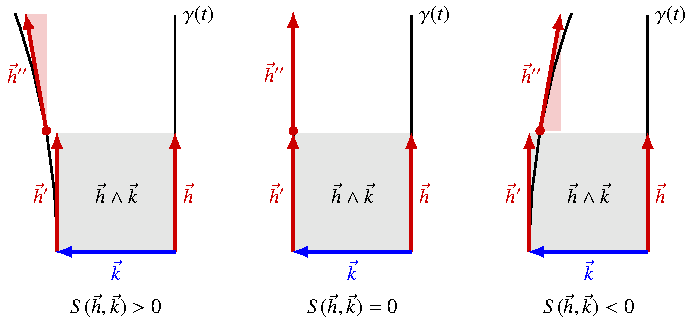
\includegraphics{chapters/110-kruemmung/images/abstand.pdf}
\caption{Schnittkrümmung und der Abstand von Geodäten mit
parallelverschobener Anfangsrichtung, die von infinitesimal
benachbarten Punkten ausgehen.
Bei positiver Schnittkrümmung wird der Abstand grösser, bei negtiver
Schnittkrümmung wird er kleiner.
\label{buch:kruemmung:schnittkruemmung:fig:abstand}}
\end{figure}

Die Schnittkrümmung codiert auch, sich der Abstand von Geodäten,
die in geringem Abstand aber mit paralleltransportierter Richtung
beginnen.
Dazu betrachten wir eine Geodäte mit Tangente $\vec{h}$ und
vergleichen Sie mit einer Geodäte, deren Anfangspunkt infinitesimal
in Richtung $\vec{k}$ verschoben ist.

Ist die Schnittkrümmung $S(\vec{h},\vec{k})=0$, dann dreht sich der
Tangentialvektor beim Paralleltransport nicht.
In der Abbildung~\ref{buch:kruemmung:schnittkruemmung:fig:abstand}
in der Mitte wird dies dadurch angezeigt, dass der Vektor $\vec{h}''$
seine Richtung nicht geändert hat.

Bei positiver Schnittkrümmung, dargestellt in
Abbildung~\ref{buch:kruemmung:schnittkruemmung:fig:abstand}
links, dreht sich der Tangentialvektor in positiver Richtung und der
Abstand zwischen den Geodäten wird grösser.
Umgekehrt dreht sich bei negativer Schnittkrümmung, dargestellt in
Abbildung~\ref{buch:kruemmung:schnittkruemmung:fig:abstand} rechts,
der Tangentialvektor $\vec{h}''$ im Uhrzeigersinn, der Abstand
der Geodäten wird kleiner.

Man kann die Abstandsänderung auch direkt aus den Rechenregeln für
die kovariante Ableitung berechnen, für unsere Zwecke soll die
intuitive graphische Erklärung von 
Abbildung~\ref{buch:kruemmung:schnittkruemmung:fig:abstand}
genügen.

Später in Abschnitt~\ref{buch:kruemmung:section:newton} wird gezeigt,
dass die Abstandsänderung als gravitative Wirkung interpretiert
werden kann.
Damit ist bereits angedeutet, was die allgemeine Relativitätstheorie
beweist, dass nämlich Gravitation durch die Krümmung der Raum-Zeit
beschrieben werden kann.

%
% Schnittkrümmungen bestimmen den riemannschen Krümmungstensor
%
\subsection{Schnittkrümmungen bestimmen den riemannschen Krümmungstensor}

\begin{satz}
Der riemannsche Krümmungstensor einer Mannigfaltigkeit $M$
ist vollständig bestimmt durch die Schnittkrümmungen.
\end{satz}

Der Beweis wird zeigen, dass sich sogar eine konkrete Formel
für die Werte des Krümmungstensors angeben lässt.

\begin{proof}
Die Komponenten $R_{lhik}$ des riemannsche Krümmungstensors ist
antisymmetrisch im ersten und letzten Indexpaar.
Es gilt also
\[
R_{lhik}
-R_{hlik}
=
-R_{lhki}.
\]
Dies bedeutet, dass die 4-Linearform
\[
Rm(X,Y,Z,W)
=
\xi^l\eta^h\zeta^i\omega^k R_{lhik}
\]
nur von den 2-Vektoren $X\wedge Y$ bzw.~$Z\wedge W$ abhängt.
Der Krümmungstensor kann daher auch als blineare Funktion
\begin{equation}
\bigwedge^2 TM\otimes\bigwedge^2 TM
\to
\mathbb{R}
:
(X\wedge Y,Z\wedge W)
\mapsto
R(X\wedge Y, Z\wedge W)
=
Rm(X,Y,Z,W)
\label{buch:kruemmung:schnittkruemmung:eqn:Rbivektor}
\end{equation}
auf dem Vektorraum $\bigwedge^2 TM$ der 2-Vektoren von Tangentialvektoren
geschrieben werden.

Der Krümmungstensor ist ausserdem symmetrisch unter der Vertauschung
der Indexpaare $lh$ und $ik$.
Dies bedeutet, dass die
in
\eqref{buch:kruemmung:schnittkruemmung:eqn:Rbivektor}
definierte Funktion $R$ auf den 2-Vektoren symmetrisch ist:
\begin{align*}
R(X\wedge Y,Z\wedge W)
=
R(Z\wedge W,X\wedge Y)
\end{align*}
für beliebige 2-Vektoren $X\wedge Y,Z\wedge W\in\bigwedge^2TM$.
Wir schreiben die symmetrische, bilineare Funktion auch als $R(u,v)$ mit
$u,v\in\bigwedge^2 TM$.

Wir möchten zeigen, dass sich $R(u,v)$ aus den Werten $R(w,w)$ für beliebige
2-Vektoren $w$ berechnen lässt.
Um dies etwas prägnanter auszudrücken, schreiben wir
\[
Q(w) = R(w,w).
\]
Die Funktion $Q$ ist eine quadratische Form.

Die Polarisationsformel \cite[p. 347]{buch:linalg} besagt, dass eine
symmetrische, bilineare Funktion $R(u,v)$ vollständig durch die
Werte $R(u,v)$ bestimmt ist.
Wir führen die Rechnung 
\begin{align}
R(u+v,u+v)
&=
R(u,u) + R(u,v) + R(v,u) + R(v,v)
\notag
\\
\Rightarrow\qquad
Q(u+v)
&=
R(u,u) + 2R(u,v) + R(v,v)
\notag
\\
R(u-v,u-v)
&=
R(u,u) - R(u,v) - R(v,u) + R(v,v)
\notag
\\
\Rightarrow\qquad
Q(u-v)
&=
R(u,u) - 2R(u,v) + R(v,v)
\notag
\intertext{mit der Differenz}
Q(u+v)-Q(u-v)
&=
4 R(u,v),
\notag
\intertext{oder aufgelöst nach dem gemischten Term:}
R(u,v)
&=
{\textstyle\frac14}\bigl( Q(u+v) - Q(u-v) \bigr).
\label{buch:kruemmung:schnittkruemmung:eqn:RQQ}
\end{align}
Die Formel \eqref{buch:kruemmung:schnittkruemmung:eqn:RQQ}
drückt $R(u,v)$ durch Werte der Form $R(w,w)$ mit $w\in\bigwedge^2 TM$ aus.
\end{proof}

\begin{satz}
Der Krümmungstensor ist durch die Schnittkrümmungen vollständig
bestimmt.
\end{satz}

\begin{proof}
Die Schnittkrümmung zu den Vektoren $\vec{s}$ und $\vec{v}$ ist
definiert durch
\begin{align}
K(\vec{s},\vec{v})
&=
\frac{
R(\vec{v},\vec{s},\vec{v},\vec{s})
}{
|\vec{v}\wedge\vec{s}|^2
}.
\intertext{Für einen Basis-2-Vektor $\vec{e}_i\wedge\vec{e}_k$ wird dies zu}
K(\vec{e}_i,\vec{e}_k)
&=
\frac{Rm(\vec{e}_i,\vec{e}_k,\vec{e}_i,\vec{e}_k)}{|\vec{e}_i\wedge\vec{e}_k|^2}
\notag
\\
&=
\frac{R_{ikik}}{g^{ii}g^{kk}-g^{ik}g^{ik}}.
\label{buch:kruemmung:schnittkruemmung:eqn:Rgggg}
\end{align}
Da $g$ als Metrik definit ist, ist der Nenner von
\eqref{buch:kruemmung:schnittkruemmung:eqn:Rgggg}
niemals 0.
Der Riemannsche Krümmungstensor kann also aus den Werten
\[
Rm(\vec{e}_i,\vec{e}_k,\vec{e}_i,\vec{e}_k)
=
R(\vec{e}_i\wedge\vec{e}_k,\vec{e}_i\wedge\vec{e}_k)
=
Q(\vec{e}_i\wedge\vec{e}_k)
=
(g^{ii}g^{kk}-g^{ik}g^{ik}) K(\vec{e}_i,\vec{e}_k)
\]
bestimmt werden.
Sie können also aus den Schnittkrümmungen ermittelt werden.
\end{proof}

Der Satz besagt also, dass die vom riemannschen Krümmungstensor
beschriebene Krümmung des Raumes vollständig ergründet werden kann,
indem man Messungen in divergierenden Gedäten durchführt.
Eine andere Art, dies auszudrücken, ist, dass der riemannsche
Krümmungstensor keine zusätzliche Information erhält, die man nicht
in der Funktion der Schnittkrümmungen gefunden werden kann.

%
% Ricci-Krümmung
%
\section{Ricci-Krümmung
\label{buch:kruemmung:section:ricci}}
\kopfrechts{Ricci-Krümmung}
%
% fig-schnittkruemmung.tex
%
% (c) 2025 Prof Dr Andreas Müller
%
\begin{figure}
\centering
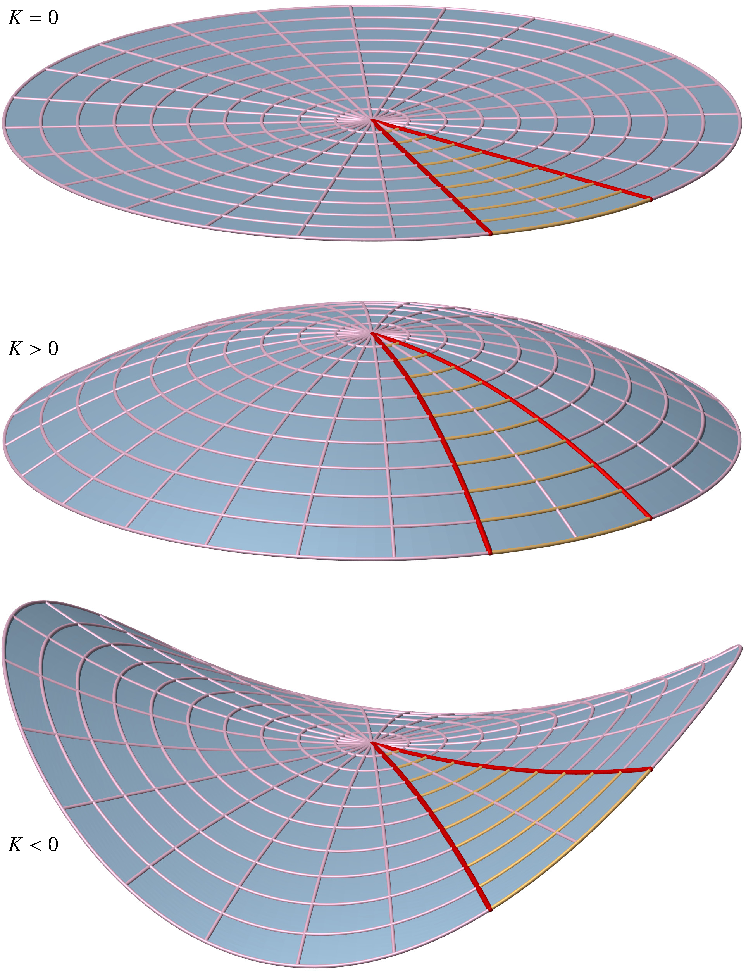
\includegraphics{chapters/110-kruemmung/images/kruemmung.pdf}
\caption{Die Schnittkrümmung bestimmt, wie schnell sich Geodäten
voneinander entfernen.
Der Abstand der Geodäten wächst linear mit dem Radius, wenn 
$K=0$ ist, der Abstand wächst schneller als linear für $K<0$ und
langsamer als linear für $K>0$.
\label{buch:kruemmung:fig:schnittkruemung}}
\end{figure}

Die Komponente $R^l\mathstrut_{ijk}$  des Riemann-Krümmungstensors
beschreibt, wie sich die $l$-Komponente des des $i$-ten 
Standardbasisvektors $\vec{e}_i$ beim Paralleltransport um
ein infinitesmales Quadrat mit dem 2-Vektor $\vec{e}_j\wedge \vec{e}_k$
verändert.
Für die physikalische Interpretation des Gravitationsfeldes ist
es wichtig zu verstehen, wie sich der Abstand von Geodäten mit
ähnlichen Anfangsbedingungen verändert, da wir dies als relative
Beschleunigung und damit als Anziehungs- oder Abstossungskraft 
interpretieren können.

%
% Der Ricci-Tensor
%
\subsection{Der Ricci-Tensor}
Der riemannsche Krümmungstensor wurde mit der linearen Abbildung
$R(X,Y)$ definiert, die ihrerseits durch
\[
R(X,Y)Z
=
\nabla_X\nabla_YZ - \nabla_Y\nabla_XZ-\nabla_{[X,Y]}Z
\]
definiert war.
Hält man $Y$ und $Z$ fest, ist $f:X\mapsto R(X,Y)Z$ eine lineare Abbildung.
Die Abbildung hängt ausserdem linear von den Vektoren $Y$ und $Z$ ab.

In einem Koordinatensystem $x^i$ ist die
Abbildung für $Y=\partial_k$ und $Z=\partial_l$  gegeben durch
\[
\partial_i
\mapsto
R(\partial_i,\partial_k)\partial_l
\]
Die Matrixelemente können daraus mithilfe des Skalarprodukts mit
einem Basisvektor ermittelt werden.
Die Basisvektoren werden gemäss
\[
\partial_i
\mapsto
\langle
R(\partial_i,\partial_k)\partial_l,
\partial_m
\rangle
=
R^{m}\mathstrut_{lik}\partial_m
\]
abgebildet.
Für die genannte spezielle Wahl von $Y$ und $Z$ sind also die 
die Matrixelemente von der Abbildung durch Komponenten des
riemannschen Krümmungstensors gegeben sind.
Die Matrix der Abbildung ist
\[
A^m\mathstrut_i
=
\begin{pmatrix}
R^1\mathstrut_{l1k} & R^1\mathstrut_{l2k} & \dots  & R^1\mathstrut_{lnk} \\
R^2\mathstrut_{l1k} & R^2\mathstrut_{l2k} & \dots  & R^2\mathstrut_{lnk} \\
\vdots              & \vdots              & \ddots & \vdots              \\
R^n\mathstrut_{l1k} & R^n\mathstrut_{l2k} & \dots  & R^n\mathstrut_{lnk} 
\end{pmatrix}.
\]
Um mehr über diese Abbildung zu erfahren, kann man bekannte
Invarianten linearer Abbildungen studieren.
Die Spur einer linearen Abbildung ist die Summe der Diagonalelemente,
also
\[
\operatorname{tr} A^m\mathstrut_i
=
\sum_{i=1}^n A^i\mathstrut_i.
\]
Es ist ein bekanntes Resultat der linearen Algebra, dass die Spur
unabhängig ist von der Wahl des Koordinatensystems.
Es folgt aus der Tatsache, dass ein Basiswechsel durch ein
Transformationsmatrix $T$ gegeben wird, mit der die Matrix der
Abbildung in der neuen Basis durch $A'=TAT^{-1}$ berechnet
werden kann.
Der Wert der Spur ist dann
\[
\operatorname{tr} A'
=
\operatorname{tr}(TAT^{-1})
=
\operatorname{tr}(A\underbrace{T^{-1}T}_{\displaystyle=I})
=
\operatorname{tr}A.
\]
Der Wert der Spur hängt also nicht von der Wahl der Basis ab.
Die Spur ist somit eine von der Wahl des Koordinatensystems
unabhängige Grösse, die bilinear von den Vektoren $Y$ und $Z$
abhängt.

\begin{definition}[Ricci-Tensor]
Der \emph{Ricci-Tensor} $Ric(Y,Z)$ ist die Spur der linearen Abbildung
\[
X \mapsto R(X,Y)Z = (\nabla_X\nabla_YZ-\nabla_Y\nabla_XZ-\nabla_{[X,Y]}Z.
\]
Für $Y=y^l\partial_l$ und $Z=z^k\partial_k$ ist der Wert der Spur
durch die Bilinearform
\[
Ric(Y,Z)
=
R^m\mathstrut_{lmk} y^lz^k
=
g^{im}
R_{ilmk}y^lz^k
\]
gegeben.
Die Komponenten des Ricci-Tensors sind also
\[
Ric(\partial_l,\partial_k)
=
R_{lk}
=
R^m\mathstrut_{lmk}
=
g^{im}
R_{ilmk}.
\]
\end{definition}

%
% Symmetrie
%
\subsubsection{Symmetrie}
Der Ricci-Tensor ist ein symmetrischer Tensor, wie man zum Beispiel
durch Anwendung der Symmetrieeigenschaften des riemannschen Krümmungstensors
in
\[
R_{kl}
=
g^{im}R_{ilmk}
=
g^{im}R_{mkil}
=
g^{im}R_{mkil}
=
g^{im}R_{ikml}
\]
sehen kann.
Im zweiten Schritt wurde die Symmetrie unter Vertauschung der beiden
Indexpaare verwendet, im dritten die Symmetrie des metrischen Tensors
und im letzten wurden die summierten Indizes umbenannt.

%
% Ricci-Tensor in Normalkoordinaten
%
\subsection{Ricci-Tensor in Normalkoordinaten}
In Normalkoordinaten kann man die Komponenten des Ricci-Tensors
nach \eqref{buch:kruemmung:kruemmung:eqn:Rruvm} im Punkt $p$ durch
\begin{align*}
R_{lk}
&=
g^{im}
R_{ilmk} 
\\
&=
\delta^{im}
\biggl(
\frac{\partial \Gamma^i_{lm}}{\partial x^k}
-
\frac{\partial \Gamma^i_{lk}}{\partial x^m}
\biggr)
\\
&=
\frac{\partial \Gamma^m_{lm}}{\partial x^k}
-
\frac{\partial \Gamma^m_{lk}}{\partial x^m}
\intertext{berechnen.
Da man ausserdem die Ableitungen der Christoffel-Symbole durch zweite
Ableitungen der metrischen Koeffizienten ausdrückenkann, kann man
den Ricci-Tensor mithilfe von \eqref{buch:kruemmung:kruemmung:eqn:Rddg}
auch als}
R_{lk}
&=
g^{im}
R_{ilmk} 
\\
&=
\delta^{im}
\frac12
\biggl(
\frac{\partial^2 g_{im}}{\partial x^k\,\partial x^l}
-
\frac{\partial^2 g_{lm}}{\partial x^k\,\partial x^i}
-
\frac{\partial^2 g_{ik}}{\partial x^m\,\partial x^l}
+
\frac{\partial^2 g_{lk}}{\partial x^m\,\partial x^i}
\biggr)
\\
&=
\frac12
\sum_{m=1}^n
\biggl(
\frac{\partial^2 g_{mm}}{\partial x^k\,\partial x^l}
-
\frac{\partial^2 g_{lm}}{\partial x^k\,\partial x^m}
-
\frac{\partial^2 g_{mk}}{\partial x^m\,\partial x^l}
+
\frac{\partial^2 g_{lk}}{\partial (x^m)^2}
\biggr)
\end{align*}
schreiben.
Der letzte Term dieses Ausdrucks erinnert an den Laplace-Operator,
angewendet auf alle Komponenten.

Tatsächlich ist eine Anwendung des Ricci-Tensors die Definition einer
Differentialgleichung für den metrischen Tensor auf einer riemannsche
Mannigfaltigkeit, die der Wärmeleitung ähnlich ist.
Die Zeitentwicklung der Lösung, der sogenannte Ricci-Fluss, deformiert
die Krümmung derart, dass die Krümmung reduziert wird, so wie die
Wärmeleitungsgleichung die Temperaturverteilung glättet.
Mit diesem Werkzeug wurde es möglich, die Poincaré-Vermutung, eines
der berühmten Millenniumsprobleme zu lösen.


%
% Krümmungsskalar
%
\subsection{Krümmungsskalar}
Die Spur des Ricci-Tensors 
\[
S
=
g^{ik}R_{ik}
=
R^i_k
\]
ist ebenfalls eine koordinatensystemunabhängige Grösse, sie
heisst der {\em Krümmungsskalar}.
\index{Krummungsskalar@Krümmungsskalar}
Der Krümmungsskalar ist als Tensor nullter Stufe eine weitere Invariante,
die in einer Feldgleichung für die Gravitation vorkommen könnte.

Der Tensor $Sg$ mit den Komponenten $Sg_{ik}$ hat die Spur
\[
\operatorname{tr} Sg
=
Sg^{ik}g_{ik}
=
nS.
\]
Daher ist $\frac1n Sg$ ein symmetrischer Tensor mit der gleichen
Spur wie der Ricci-Tensor. 
Wir bezeichnen mit
\[
\overset{\circ}{Ric}
=
Ric - \frac1n Sg
\]
den \emph{spurlosen Ricci-Tensor}.

Die besondere Bedeutung des Krümmungsskalars ist, dass die Zerlegung
\begin{equation}
Ric
=
\overset{\circ}{Ric} + \frac1n Sg
\label{buch:kruemmung:ricci:eqn:Riczerlegung}
\end{equation}
orthogonal ist.

\begin{satz}
Die Zerlegung \eqref{buch:kruemmung:ricci:eqn:Riczerlegung} ist
orthogonal, d.~h.~der spurlose Ricci-Tensor $\overset{\circ}{Ric}$
und $\frac1nSg$ sind orthogonal.
\end{satz}

\begin{proof}
Sei $h$ ein beliebiger symmetrischer Tensor mit Komponenten $h_{ik}$,
dann ist das Skalarprodukt mit dem metrischen Tensor mit den 
Komponenten $g_{lm}$ durch
\begin{align*}
\langle h,g\rangle
&=
h_{ik}g_{lm}
g^{il}g^{km}
=
h_{ik}\delta_m^i
g^{km}
=
h_{ik}g^{ik}
=
\operatorname{tr} h
\end{align*}
gegeben.
Daher ist das Skalarprodukt
\[
\langle \overset{\circ}{Ric},\frac{1}n Sg \rangle
=
\frac1nS\langle\overset{\circ}{Ric},g\rangle
=
\frac1nS\operatorname{tr}\overset{\circ}{Ric}
=
0,
\]
die Tensoren $\overset{\circ}{Ric}$ und $\frac1nSg$ sind orthogonal.
\end{proof}

Die äussere Ableitung des Krümmungsskalars kann durch Kontraktion
der kovarianten Ableitung des Ricci-Tensors gewonnen werden.

%
% Kontrahierte Bianchi-Identitäten
%
\subsection{Kontrahierte Bianchi-Identitäten}
Der Ricci-Tensor entsteht durch Kontraktion zweier Indizes aus dem
riemannschen Krümmungstensor gewonnen.
Die Bianchi-Identitäten müssen sich daher auch in Identitäten
für den Ricci-Tensor äussern.
Wir berechnen diese Identitäten zunächst in Komponenten, bevor wir
eine koordinatenfreie Beschreibung geben.

%
% Kontrahierte algebraische Bianchi-Identität
%
\subsubsection{Kontrahierte algebraische Bianchi-Identität}
Die algebraische Bianchi-Identität besagt, dass
\[
0
=
R_{iklm}
+
R_{ilmk}
+
R_{imkl}
\]
Multiplikation mit $g^{il}$ wird daraus
\begin{align*}
0
&=
R_{km}
+
g^{il}R_{ilmk}
+
g^{il}R_{imkl}.
\intertext{Der mittlere Term verschwindet, weil der riemannsche
Krümmungstensor in den ersten beiden Indizes $il$ antisymmetrisch ist,
während $g^{il}$ symmetrisch ist.
Im letzten Term können wir die letzten zwei Indizes vertauschen, was
das Vorzeichen kehrt.
So entsteht}
&=
R_{km}
-
g^{il}R_{imlk}
\\
&=
R_{km}-R_{mk}.
\end{align*}
Die erste Bianchi-Identität liefert also nichts anderes als die
Symmetrie des Ricci-Tensors, die wir bereits kennen.

%
% Kontrahierte differentielle Bianchi-Identität
%
\subsubsection{Kontrahierte differentielle Bianchi-Identität}
Wir wenden die Kontraktion auch auf die differentielle Bianchi-Identität
\[
0
=
R_{abik;l}
+
R_{abkl;i}
+
R_{abli;k}
\]
an und erhalten
\begin{align}
0
&=
g^{ai}
(
R_{abik;l}
+
R_{abkl;i}
+
R_{abli;k}
)
\notag
\\
&=
R_{bk;l}
+
g^{ai}
R_{abkl;i}
+
g^{ai}
R_{abli;k}
\notag
\\
&=
R_{bk;l}
+
g^{ai}
R_{abkl;i}
-
g^{ai}
R_{abil;k}
\notag
\\
&=
R_{bk;l}
+
g^{ai}
R_{abkl;i}
-
R_{bl;k}
\notag
\\
R^i\mathstrut_{bkl;i}
&=
-(
R_{bk;l}
-
R_{bl;k}
)
\label{buch:kruemmung:ricci:eqn:kontrdbianchi}
\end{align}
Die Formel \eqref{buch:kruemmung:ricci:eqn:kontrdbianchi} kann
man noch in eine koordinatenfreie Form bringen und damit besser
verstehen.
Hält man in $\overset{\circ}{Ric}(X,Y)$ einen der Vektor fest,
entsteht eine $1$-Form.
Der Ricci-Tensor kann also als eine 1-Form mit Werten in 
1-Formen betrachten.
Wir schreiben $\boldsymbol{\alpha}$ für die 1-Form $X\mapsto R(X,Y)$
und berechnen die kovariante äussere Ableitung.
Sie erfüllt
\begin{align*}
\langle \boldsymbol{d}\boldsymbol{\alpha}, Y\wedge Z\rangle
&=
\nabla_Y\langle\boldsymbol{\alpha},Z\rangle
-
\nabla_Z\langle\boldsymbol{\alpha},Y\rangle
-
\langle \boldsymbol{\alpha}, [Y,Z] \rangle
\intertext{Auf dem Vektor $X$ hat diese 1-Form den Wert}
\langle\boldsymbol{d}\boldsymbol{\alpha},Y\wedge Z\rangle (X)
&=
\nabla_Y {Ric}(X,Z)
-
\nabla_Z {Ric}(X,Y)
-
{Ric}(X,[Y,Z])
\end{align*}
Setzt man für die Vektoren $X$, $Y$ und $Z$ die Standardbasisvektoren
$\partial_b$, $\partial_k$ und $\partial_l$ ein, wird daraus
\begin{align*}
\langle\boldsymbol{d}\boldsymbol{\alpha},\partial_k\wedge \partial_l\rangle
(\partial_b)
&=
\nabla_k {Ric}(\partial_b,\partial_l)
-
\nabla_l {Ric}(\partial_b,\partial_k)
-
{Ric}(\partial_b,[\partial_k,\partial_l]).
\intertext{Weil die Basisoperatoren $\partial_i$ vertauschen ist
$[\partial_k,\partial_l])=0$ und der letzte Term fällt weg.
Es bleibt}
&=
\nabla_k {Ric}(\partial_b,\partial_l)
-
\nabla_l {Ric}(\partial_b,\partial_k)
=
R_{bl;k}
-
R_{bk;l}
\end{align*}
Die kontrahierte differentielle Bianchi-Identität sagt also, dass
die Spur der kovarianten Ableitung des riemannschen Krümmungstensors
die kovariante äussere Ableitung des Ricci-Tensors ist.




%
% Newtonsche Gravitation als Raumkrümmung
%
\section{Newtonsche Gravitation als Raumkrümmung
\label{buch:kruemmung:section:newton}}
\kopfrechts{Newtonsche Gravitation als Raumkrümmung}
Es gehört schon fast zum Allgemeinwissen, dass die einsteinsche
Relativitätstheorie die Gravitation als Raumkrümmung beschreibt.
Tatsächlich erlaubt aber auch die newtonsche Theorie eine solche
Interpretation, wie in diesem Abschnitt gezeigt werden soll.

%
% Koordinatensystem und newtonsche Gravitation
%
\subsection{Koordinatensystem und newtonsche Gravitation}
Wir verwenden ein vierdimensionales Koordinatensystem mit
den Koordinaten $x^0=ct$, $y^1=x$, $x^2=y$ und $x^3=z$.
Die Bahn eines Teilchens im Gravitationsfeld eines Himmelskörpers
der Masse $M$, der sich im Nullpunkt des Koordinatensystems befindet,
ist dann durch die Funktion
\[
t\mapsto
\begin{pmatrix}
ct\\
x(t)\\
y(t)\\
z(t)
\end{pmatrix}
\]
gegeben, die die Differentialgleichung
\begin{equation}
\frac{d^2}{dt^2}
\begin{pmatrix}
ct\\
x(t)\\
y(t)\\
z(t)
\end{pmatrix}
=
\begin{pmatrix}
0\\
\ddot{x}(t)\\
\ddot{y}(t)\\
\ddot{z}(t)
\end{pmatrix}
=
-
\frac{GMm}{r(t)^3}
\begin{pmatrix}
0\\
x(t)\\
y(t)\\
z(t)
\end{pmatrix}
\label{buch:kruemmung:newton:eqn:dgl}
\end{equation}
erfüllt, wobei
\[
r(t)
=
\sqrt{x(t)^2 + y(t)^2 + z(t)^2}
\]
ist.
Es ist möglich, die Bahn im Gravitationsfeld eines einzelnen,
ruhenden Himmelskörpers in geschlossener Form zu lösen.
Sobald mehrere massereiche Himmelskörper die Bahn beeinflussen,
wie dies im Sonnensystem mit dem Einfluss des Planeten Jupiter
\index{Sonnensystem}%
\index{Jupiter}%
der Fall ist, sind nur noch numerische Lösungen möglich.
Daher wird im folgenden nicht versucht, Lösungen direkt miteinander
zu vergleichen.
Stattdessen soll gezeigt werden, dass die Differentialgleichung
\eqref{buch:kruemmung:newton:eqn:dgl}
auch als Geodätengleichung einer geeigneten Metrik geschrieben
werden kann.
Zu diesem Zweck schreiben wir die Differentialgleichung noch in
der Komponentenform
\begin{equation}
\begin{aligned}
\ddot{x}^0(t) &= 0 \\
\ddot{x}^i(t) &= - \frac{GM}{r(t)^2}\,x^i(t)\qquad \text{für $i>0$}.
\end{aligned}
\label{buch:kruemmung:newton:eqn:dglcomponents}
\end{equation}
Die erste Gleichung bedeutet nichts anderes, als dass es in der
newtonschen Gravitationstheorie eine absolute Zeit gibt.
\index{Gravitation!newtonsch}%

%
% Gravitationspotential
%
\subsection{Gravitationspotential}
Das newtonsche Gravitationsfeld ist ein Potentialfeld.
Das Potential der Masse $M$ im Nullpunkt des Koordinatensystems
hat das Potential
\[
U(x) = \frac{GM}{r}.
\]
\index{Gravitationspotential}%
Tatsächlich ist der Gradient 
\[
\operatorname{grad}U
=
-\frac{GM}{r^2} \operatorname{grad}{r}
=
-\frac{GM}{r^2}
\cdot
\frac{1}{2r}
\begin{pmatrix}
2x(t)\\
2y(t)\\
2z(t)
\end{pmatrix}
=
-\frac{GM}{r^3}
\begin{pmatrix}
x(t)\\
y(t)\\
z(t)
\end{pmatrix}
.
\]
Die rechte Seite stimmt mit der rechten Seite der Differentialgleichung
\eqref{buch:kruemmung:newton:eqn:dgl}
überein.

Sind mehrere Massepunkte gegeben, kann ihr gemeinsames Potential 
als Summe
\[
U(x)
=
\sum_{i=1}^n U_i(x)
\]
geschrieben werden, wobei
\[
U_i(x)
=
\frac{GM_i}{|x-x_i|}
\]
das Potential der Masse $M_i$ an der Stelle $x_i$ ist.

Für die folgende Rechnung gehen wir von der Annahme aus, dass sich die
Massen nicht bewegen, dass das Gravitationsfeld also statisch ist.
Diese Annahme ist näherungsweise dadurch gerechtfertigt, dass die
Geschwindigkeit der Massen in schwachen Gravitationsfeldern wie in
unserem Sonnensystem viel kleiner sind als die Lichtgeschwindigkeit.

%
% Metrik
%
\subsection{Metrik}
Wir verwenden die Metrik
\begin{equation}
\begin{aligned}
g_{00} &= \phantom{-}1 + \frac{2U(x)}{c^2} \\
g_{ii} &= -1\qquad &i&>0
\end{aligned}
\label{buch:kruemmung:newton:eqn:metrik}
\end{equation}
für die vierdimensionale Mannigfaltigkeit mit den Koordinaten
$(x^0,x^1,x^2,x^3)$.
Nur die Zeitkomponente der Metrik weicht von der Minkowski-Metrik ab.
\index{Minkowski-Metrik}%

Da das Potential im Vergleich zu $c^2$ klein ist, werden wir nur in
erster Näherung arbeiten.
Terme zweiter Ordnung in $U/c^2$ enthalten Quadrate von $U/c^2$ und sind
noch viel kleiner, sie dürfen daher vernachlässigt werden.

In den folgenden Abschnitten werden schrittweise die Christoffel-Symbole
berechnet, mit denen dann in
Abschnitt~\ref{buch:kruemmung:newtion:subsection:geodaeten}
die Geodätengleichung aufgestellt werden soll.

%
% Die Inverse der Metrik
%
\subsubsection{Die Inverse der Metrik}
Da die Metrik im gewählten Koordinatensystem eine Diagonalmatrix ist,
ist auch die inverse Matrix diagonal mit den reziproken Diagonalelementen.
Wir brauchen nur eine Approximation in erster Ordnung in $2U/c^2$
für diese Elemente.

Das Element $g_{00}$ ist von der Form $1+x$.
Die geometrische Reihe
\[
1+q+q^2+q^3+\dots = \frac{1}{1-q}
\]
liefert für $q=-x$ die Approximation
\[
\frac{1}{1+x} = 1-x+x^2-x^3+o(x^3)
\]
für das reziproke Element.
Angewendet auf den Tensor $g_{ik}$ ergeben sich in erster Ordnung
die Diagonalelemente
\begin{equation}
\begin{aligned}
g^{00}
&=
\frac{1}{\displaystyle 1+\frac{2U}{c^2}}
=
1-\frac{2U}{c^2}+o\biggl(\frac{2U}{c^2}\biggr)
\\
g^{ii}&= -1
&&\text{für $i>0$.}
\end{aligned}
\end{equation}

%
% Ableitung der metrischen Koeffizienten
%
\subsubsection{Ableitungen der metrischen Koeffizienten}
Da nur das Element $g_{00}$ nicht konstant ist, gibt es nur die eine
nicht verschwindende Ableitung
\[
\frac{\partial g_{00}}{\partial x^k}
=
\begin{cases}
0
&\qquad\text{für $k=0$}\\[4pt]
\displaystyle
\frac{2}{c^2}
\frac{\partial U}{\partial x^k}
&\qquad\text{für $k>0$.}
\end{cases}
\]

%
% Christoffel-Symbole 1. Art
%
\subsubsection{Christoffel-Symbole erster Art}
Die Christoffel-Symbole erster Art sind
\[
\Gamma_{l,ik}
=
\frac{1}{2}\biggl(
\frac{\partial g_{lk}}{\partial x^i}
+
\frac{\partial g_{li}}{\partial x^k}
-
\frac{\partial g_{ik}}{\partial x^l}
\biggr).
\]
Es folgt, dass nur diejenigen Christoffel-Symboel von $0$ verschieden
sind, die genau zwei $0$-Indizes haben.
Diese sind
\begin{align}
\Gamma_{l,00}
&=
-\frac12 \frac{\partial g_{00}}{\partial x^l}
=
-
\frac{1}{c^2}\frac{\partial U}{\partial x^l}
\notag
\\
\Gamma_{0,l0}
=
\Gamma_{0,0l}
&=
\phantom{-}
\frac{1}{2}\frac{g_{00}}{\partial x^l}
=
\frac{1}{c^2}\frac{\partial U}{\partial x^l},
\label{buch:kruemmung:newton:eqn:bewegungsgleichung}
\end{align}
wobei $l>0$ ist.
Alle anderen Christoffel-Symbole verschwinden.

%
% Christoffel-Symbole 2. Art
%
\subsubsection{Christoffel-Symbole zweiter Art}
Die Christoffel-Symbole zweiter Art entstehen durch Multiplikation
mit von $\Gamma_{l,ik}$ mit $g^{jl}$.
Da nur die Elemente mit $j=l$ von Null verschieden sind, sind wieder
nur die Christoffel-Symbole zweiter Art von Null verschieden, die zwei
$0$-Indizes haben:
\begin{align*}
\Gamma^l_{00}
&=
(-1)\cdot\biggl(-\frac{1}{c^2}\frac{\partial U}{\partial x^l}\biggr)
=
\frac{1}{c^2}\frac{\partial U}{\partial x^l}
\\
\Gamma^0_{l0}
=
\Gamma^0_{0l}
&=
\biggl(1-\frac{2U}{c^2}\biggr)
\frac{1}{c^2}\frac{\partial U}{\partial x^l}
=
\frac{1}{c^2}\frac{\partial U}{\partial x^l}
+
o\biggl(
\frac{2U}{c^2}
\biggr)
\end{align*}
für $l>0$.
Die nicht verschwindenden Christoffel-Symbole zweiter Art hängen nur
vom Index $l$ ab.
Abkürzend können wir
\[
\Gamma^l_{00}
=
\Gamma^0_{l0}
=
\Gamma^0_{0l}
=
\Gamma_l
= 
\frac{1}{c^2} \frac{\partial U}{\partial x^l}
\]
schreiben.

%
% Geodäten
%
\subsection{Geodäten
\label{buch:kruemmung:newtion:subsection:geodaeten}}
Die Geodätengleichung ist
\[
\frac{d^2 x^l}{ds^2}
=
-
\Gamma^l_{ik} \frac{dx^i}{ds}\frac{dx^k}{ds}.
\]
Mit den oben berechneten Werten für die Christoffel-Symbole zweiter
Art wird daraus für $l>0$ die Gleichung
\begin{align}
\frac{d^2x^l}{ds^2}
&=
-
\Gamma^l_{00}\frac{dx^0}{ds}\frac{dx^0}{ds}
=
-
\frac{1}{c^2}
\frac{\partial U}{\partial x^l}
\frac{dx^0}{ds}
\frac{dx^0}{ds}.
\notag
\intertext{
Man möchte aber $t$ als Kurvenparameter verwenden, nicht $s$, was man
durch Multiplikation mit $(ds/dt)^2$ und Anwendung der Kettenregel
erreichen kann.
Es entsteht}
\frac{d^2x^l}{ds^2}
\biggl(\frac{ds}{dt}\biggr)^2
&=
-
\frac{1}{c^2}
\frac{\partial U}{\partial x^l}
\frac{dx^0}{ds}
\frac{dx^0}{ds}
\biggl(\frac{ds}{dt}\biggr)^2
\notag
\\
\frac{d^2x^l}{dt^2}
&=
-
\frac{1}{c^2}
\frac{\partial U}{\partial x^l}
\underbrace{
\frac{dx^0}{dt}
\frac{dx^0}{dt}
}_{\displaystyle = c^2}
=
-\frac{\partial U}{\partial x^l}.
\label{buch:kruemmung:newton:geodaeten:eqn:final}
\end{align}
Dabei wurde verwendet, dass wegen $x^0=ct$ auch $dx^0/dt=c$ gilt.
\eqref{buch:kruemmung:newton:geodaeten:eqn:final}
ist die Bewegungsgleichung für die Bewegung eines Teilchens
im Gravitationspotential $U(x)$.

Die Geodätengleichung für die $0$-Komponente ist
\begin{align*}
\frac{d^2x^0}{ds^2}
&=
-
\Gamma^0_{ik}
\frac{dx^i}{ds}
\frac{dx^k}{ds}.
\end{align*}
Wegen $x^0=ct$ sagt diese Gleichung nur etwas über die Abhängigkeit 
zwischen $s$ und $t$ aus, die nicht weiter interessiert,
da in der
Bewegungsgleichung~\eqref{buch:kruemmung:newton:eqn:bewegungsgleichung}
der Parameter $s$ gar nicht mehr vorkommt.

%
% Raumkrümmung
%
\subsection{Raumkrümmung für die newtonsche Gravitation}
Die Tatsache, dass aus der Metrik
\eqref{buch:kruemmung:newton:eqn:metrik}
die
Bewegungsgleichungen~\eqref{buch:kruemmung:newton:eqn:bewegungsgleichung}
der newtonschen Gravitation entstehen, rechtfertigt die Idee, die
Gravitation als Konsequenz der Raumkrümmung zu betrachten.
\index{Raumkrümmung für newtonsche Gravitation}%

%
% Der riemannsche Krümmungstensor
%
\subsubsection{Der riemannsche Krümmungstensor}
Mit den Christoffel-Symbolen kann jetzt auch der riemannsche Krümmungstensor
berechnet werden.
Die Definition ist
\begin{equation}
R^{i}\mathstrut_{klm}
=
\frac{\partial \Gamma^i_{km}}{\partial x^l}
-
\frac{\partial \Gamma^i_{kl}}{\partial x^m}
+
\Gamma^i_{nl}
\Gamma^n_{km}
-
\Gamma^i_{nm}
\Gamma^n_{kl}.
\end{equation}
Aus den Symmetrieeigenschaften des Krümmungstensors folgt, dass die
Komponenten mit $i=k$ und $l=m$ verschwinden.
Insbesondere müssen mindestens zwei der Indizes von Null verschieden sein.
In den Produkten der Christoffel-Symbole kommen nur Terme höherer Ordnung
vor, es reicht also, die Ableitungsterme zu berücksichtigen.

Damit die partiellen Ableitungen in den ersten beiden Termen nicht
verschwinden, muss nach einer Raumvariablen abgeleitet werden und von
den anderen drei Indizes muss genau einer von Null verschieden sein.
Für $i\ne 0\ne l$ ist
\begin{align}
R^i\mathstrut_{0l0}
&=
\frac{\partial \Gamma^i_{00}}{\partial x^l}
-
\frac{\partial \Gamma^i_{k0}}{\partial x^0}
=
\frac{\partial \Gamma^i_{00}}{\partial x^l}
=
\frac{1}{c^2}
\frac{\partial^2 U}{\partial x^i\,\partial x^l}.
\label{buch:kruemmung:newton:eqn:riemann}
\end{align}
Ist ein weiterer Index von 0 verschieden, sind in den Ableitungstermen
mindestens zwei Indizes der Christoffel-Symboel von 0 verschieden.
Somit verschwinden alle diese Komponenten.

%
% Ricci-Krümmung
%
\subsubsection{Ricci-Krümmung}
Die Ricci-Krümmung entsteht durch Kontraktion des riemannschen
Krümmungstensors über den ersten und dritten Index.
Die 0-Komponente ist
\[
R_{00}
=
R^l\mathstrut_{0l0}
=
\frac{1}{c^2}
\sum_{l=1}^3
\frac{\partial^2 U}{\partial (x^l)^2}
=
\frac{1}{c^2}\Delta U.
\]
Die newtonsche Gravitationstheorie besagt, dass es einen Zusammenhang
zwischen der Materiedichte $\varrho$ und dem Potential gibt, es gilt
nämlich die Differentialgleichung
\begin{equation}
\Delta U = 4\pi \varrho.
\label{buch:kruemmung:newton:potential}
\end{equation}
ersetzt man $\varrho$ durch die zugehörige Energiedichte
$\varepsilon = \varrho c^2$, ergibt sich die Gleichung
\[
R_{00}
=
\frac{4\pi G}{c^4}\varepsilon.
\]
Damit ist die später abzuleitende einsteinsche Feldgleichung bereits
angedeutet.

Die anderen Komponenten des Ricci-Tensors sind
\begin{align}
R_{0m}
&=
R^l\mathstrut_{0lm}
=
R^0\mathstrut_{00m}
=
0
&k>0
\notag
\\
R_{km}
&=
R^l\mathstrut_{klm}
=
R^0\mathstrut_{k0m}
=
R^k\mathstrut_{0m0}
=
\frac{1}{c^2}
\frac{\partial^2 U}{\partial x^k\,\partial x^m}
&k,m&>0.
\label{buch:kruemmung:newton:Rik}
\end{align}
Der Ricci-Tensor besteht also im Wesentlichen aus den zweiten
partiellen Ableitungen des Potentials.
Eine Feldgleichung für den Ricci-Tensor ist also ein lineare
partielle Differentialgleichung zweiter Ordnung für das Potential.
Die Einstein-Gleichungen werden sich als nichtlinear herausstellen,
für die vorliegende newtonsche Näherung haben wir aber in linearer
Näherung gearbeitet, so dass das verschwinden der nichtlinearen
Terme nicht überrascht.

%
% Krümmungsskalar
%
\subsubsection{Der Krümmungsskalar}
Da die Metrik $g_{ik}$ ebenso wie $g^{ik}$ diagonal sind, werden
für den Krümmungsskalar nur die diagonalen Elemente des Ricci-Tensors
benötigt.
Da Elemente von $R_{ik}$ alle von erster Ordnung sind, kann der
zusätzliche Term in $g_{00}$ bzw.~$g^{00}$ vernachlässigt werden.
Damit ist 
\begin{align*}
R
&=
g^{ik}R_{ik}
=
g^{00}R_{00}
+
\sum_{i=1}^3
g^{ii}R_{ii}
=
\frac{1}{c^2}\Delta U
-
\frac{1}{c^2}
\sum_{i=1}^3
\frac{\partial^2 U}{\partial (x^i)^2}
=
0.
\end{align*}
Der Krümmungsskalar verschwindet also.

%
% Energie-Impuls-Tensor und die Feldgleichungen der Gravitation
%
\section{Energie-Impuls-Tensor und die Feldgleichungen der Gravitation
\label{buch:kruemmung:section:gravitation}}
\kopfrechts{Energie-Impuls-Tensor und die Feldgleichungen der Gravitation}

Der Abschnitt~\ref{buch:kruemmung:section:newton} suggeriert, dass sich
die Bewegung eines Teilchens in einem newtonschen Gravitationsfeld
vollständig durch die die Metrik und den daraus abgeleiteten riemannschen
Krümmungstensor beschreiben lässt.
Die Komponenten des Ricci-Tensors scheinen nach
\eqref{buch:kruemmung:newton:Rik} die zweiten Ableitungen des
newtonschen Gravitationspotentials zu verallgemeinern.
Newtons Gravitationsgesetzt besagt, dass das Gravitationspotential von
der Masseverteilung durch die Poisson-Gleichung
\eqref{buch:kruemmung:newton:potential}
mit der Massedichte $\varrho$ bestimmt ist.
Es ist daher zu erwarten, dass eine relativistische Gravitationstheorie
konstruiert werden kann.
Die Rolle des Gravitationsfeldes wird von der Metrik übernommen und der
Laplace-Operator wird ersetzt durch den Ricci-Tensor.
Zur Vervollständigung einer Feldgleichung braucht es aber noch einen
Term, der die Massedichte $\varrho$ verallgemeinert.

%
% Konsequenzen der allgmeinen Kovarianz
%
\subsubsection{Konsequenzen der allgemeinen Kovarianz}
Die allgemeine Kovarianz fordert, dass die konstruierte Feldgleichung
von der Wahl des Koordinatensystems unabhängig sein muss.
Sie verlangt, dass die kinetische Energie bewegter Massen ebenfalls
gravitative Wirkung entfaltet.
Die Massedichte $\varrho$ fängt jedoch nur die Ruhemasse ein.
Ein Skalar oder eine Dichte ist grundsätzlich nicht fähig, die
Relativgeschwindigkeiten zu berücksichtigen.
Die Bewegung eines Teilchens äussert sich im Impuls, den es trägt.
Der Viererimpuls eines Teilchens, der als Zeitkomponente die Energie
und als Raumkomponenten die Impulskomponenten enthält, ist ein
besserer Kandidat.
Energie kann aber auch in Form von Spannungen in einem Material 
gespeichert werden.
Solche können jedoch nur mit einem Tensor zweiter Stufe wiedergegeben
werden, im Kapitel~\ref{chapter:elastomechanik} zur Elastomechanik
ausgeführt wird.

Gesucht ist also ein Feldgesetz in der Form
\begin{equation}
\left(
\begin{minipage}{1.8cm}
\raggedright
Ausdruck in $R_{ik}$ und $S$
\end{minipage}
\right)
=
\left(
\text{Kopplungskonstante}
\right)
\cdot
\left(
\begin{minipage}{3.5cm}
\raggedright
Ausdrück für Energie, Impuls und Spannungen
\end{minipage}
\right).
\label{buch:kruemmung:feldgleichungen:eqn:schema}
\end{equation}
Die allgemeine Kovarianz verlangt, dass die Terme $R_{ik}$ und $S$
nur linear auf der linken Seite auftreten können.
Somit muss auch für die rechte Seite ein Tensor zweiter Stufe sein.

Die Kopplungskonstante gibt an, wie stark die Gravitationswirkung
der Masse ist. 
In der newtonschen Theorie ist dies die Gravitationskonstante $G$
und ist durch Messungen sehr genau bestimmt worden.

%
% Der Energie-Impuls-Tensor
%
\subsubsection{Der Energie-Impuls-Tensor}
Gesucht ist daher ein Tensor $T$ zweiter Stufe mit Komponenten
$T_{ik}$, der als $T_{00}$-Komponente die Ruheenergie des enthält.
Die Komponenten $T_{0k}$ mit $k>0$ beschreiben die Impulsdichte.
Die Komponenten $T_{ik}$ mit $i,k>0$ bieten genügend Platz, die
Spannungen unterzubringen.
Auf der Diagonalen stehen die Druckspannungen, ausserhalb der Diagonalen
die Scherspannungen.
So entsteht der sogenannte \emph{Energie-Impuls-Tensor} $T$,
den man in Matrixform als
\begin{equation}
T_{ik}
=
\begin{pmatrix}
\varrho     c^2 & \varrho v_0 c & \varrho v_y c & \varrho v_z c \\
\varrho v_x c   & p_x           & \sigma_{xy}   & \sigma_{xz}   \\
\varrho v_y c   & \sigma_{yx}   & p_y           & \sigma_{yz}   \\
\varrho v_z c   & \sigma_{yx}   & \sigma_{zy}   & p_z
\end{pmatrix}
\label{buch:kruemmung:feldgleichung:eqn:Tik}
\end{equation}
schreiben kann.
Er konsolidiert auf allgemein kovariante Art alle Formen von Energie
in einem einzigen Tensor.

Da der Ricci-Tensor symmetrisch ist, muss auch der Tensor $T_{ik}$
symmetrisch sein, wenn eine lineare Feldgleichung aus dem Ricci-Tensor
und dem Energie-Impuls-Tensor gelten soll.
Die Definition \eqref{buch:kruemmung:feldgleichung:eqn:Tik} zeigt,
ist nach Konstruktion symmetrisch.
Für die Impulskomponenten ist dies offensichtlich.
Für die Spannungskomponenten beruht dies auf der in der
Elastiztitätstheorie (Kapitel~\ref{chapter:elastomechanik})
diskutierten Tatsache, dass ein asymmetrischer Spannungstensor dazu
führen würde, dass das Medium durch verbleibende Drehmomente zu
beliebig schneller Rotation angeregt würde, was nicht sein kann.

Auch das elektromagnetische Feld kann gravitative Wirkung haben.
Es gibt daher auch einen Energie-Impuls-Tensor für das elektromagnetische
Feld, der sich aus dem Faraday-Tensor konstruieren lässt, der in
Kapitel~\ref{chapter:maxwell} erklärt wird.
Er ist
\[
T^{ik}
=
F^{il}F_l\mathstrut^k - \frac12 g^{ik}F^{ab}F_{ab}.
\]
Auch dieser Tensor hat verschwindende kovariante Divergenz.

%
% Erhaltungssätze
%
\subsubsection{Erhaltungssätze}
Sowohl der Ricci-Tensor wie auch der Krümmungsskalar können in einem
Gravitationsgesetz der Form \eqref{buch:kruemmung:feldgleichungen:eqn:schema}
auftreten.
Auf der linken Seite einer Feldgleichung für die Gravitation könnten daher
eine beliebige Linearkombination $\alpha R_{ik}+\beta Sg_{ik}$ stehen.
Der Faktor $g_{ik}$ ist notwendig, um aus dem Krümmungsskalar $S$ einen
Tensor zweiter Stufe zu machen.

Der Energie-Impuls-Tensor auf der rechten Seite der Gleichung schränkt
die Linearkombination weiter ein.
Die Energieerhaltung bedeutet, dass für $T_{ik}$ eine kovariante 
Kontinuitätsgleichung gilt, die in Komponenten durch die kovariante
Divergenz
\[
T^i\mathstrut_{k;i}
=
0
\]
gegeben ist.
Der Linearkombination auf der linken Seite der Feldgleichung muss daher
ebenfalls verschwindende Divergenz haben.

Die Komponenten $R^i\mathstrut_{k;i}$ verschwinden nicht unbedingt,
es gelten die kontrahierten Bianchi-Identitäten.
Ebensowenig verschwinden die kovarianten Ableitungen $S_{;k}$.
Gesucht ist daher eine Linearkombination von $R_{ik}$ und $Sg_{ik}$,
deren kovariante Divergenz verschwindet.
Die kontrahierten Bianchi-Identitäten für den Ricci-Tensor zeigen, dass  der
\emph{Einstein-Tensor}
\index{Einstein-Tensor}%
\[
G_{ik}
=
R_{ik}
-\frac12 g_{ik}S
\]
diese Eigenschaft hat, denn in
\[
G^i\mathstrut_{k;i}
=
R^i\mathstrut_{k;i}
-
\frac12 S_{;k}
\]
ist der erste Term auf der rechten Seite
nach \eqref{buch:kruemmung:eqn:kontrahiertS}
die halbe Ableitung des Krümmungsskalars, hebt sich also mit dem
zweiten Term weg und ergibt $G^i\mathstrut_{k;i}=0$.

%
% Die Feldgleichungen
%
\subsubsection{Die Feldgleichungen}
Die Form der gesuchten Feldgleichungen der Gravitations zeichnet sich
jetzt klar ab.
Es muss nur noch die Kopplungskonstante ermittelt werden.
Durch Vergleichung mit der newtonschen Theorie schwacher Felder 
kann man zeigen, dass 
\begin{equation}
G_{ik}
=
R_{ik}
-
\frac12 Rg_{ik}
=
\frac{8\pi G}{c^4}T_{ik}
\label{buch:kruemmung:feldgleichung:eqn:feldgleichung}
\end{equation}
gelten muss.
Dies sind die \emph{einsteinschen Feldgleichungen} der Gravitation.
\index{Feldgleichung!einsteinsche}%
\index{Gravitation, Feldgleichung}%
Die folgenden Abschnitte enthalten Anwendungen auf schwarze Löcher
und die Kosmologie.


%
% Schwarze Löcher
%
\section{Schwarze Löcher und die Schwarzschild-Metrik
\label{buch:kruemmung:section:schwarzesloch}}
\kopfrechts{Schwarze Löcher und die Schwarzschild-Metrik}
Mit der Aufstellung der Feldgleichungen stellt sich sofort die Frage
nach Lösungen derselben.
Da die Feldgleichungen nichtlineare partielle Differentialgleichungen
zweiter Ordnung sind ist nicht zu erwarten, dass Lösungen ohne
zusätzliche Annahmen leicht zu finden sind.

%
% Die Schwarzschild-Metrik
%
\subsection{Die Schwarzschild-Metrik}
Eine naheliegende vereinfachende Annahme ist das Gravitationsfeld
eines kugelsymmetrischen Körpers, zum Beispiel eines nicht oder nur
sehr langsam rotierenden und zeitlich unveränderlichen Sterns.
Der Kugelsymmetrie mit mit dem Ursprung im Mittelpunkt des Sterns
tragen die Kugelkoordinaten $(r,\vartheta,\varphi)$ im Raum Rechnung.
Die Metrik darf in diesem Fall nur von der $r$-Koordinate abhängen.

Bereits einen Monat nach der Veröffentlichung von Einsteins Arbeit
über die allgemeine Relativitätstheorie hat Karl Schwarzschild
\index{Schwarzschild, Karl}%
die Lösung
\begin{equation}
ds^2
=
\biggl( 1-\frac{r_s}{r} \biggr)
c^2\,dt^2
-
\biggl(1-\frac{r_s}{r}\biggr)^{-1}
\,dr^2
-r^2 (d\vartheta^2 + \sin^2\vartheta\,d\varphi^2),
\label{buch:kruemmung:blackhole:eqn:schwarzschild}
\end{equation}
die sogenannte \emph{Schwarzschild-Metrik}
\index{Schwarzschild-Metrik}%
gefunden.
Die Koordinatenlinien sind orthogonal, da die ausserdiagonalen Elemente
des metrischen Tensors in diesen Koordinaten verschwinden.
Die Determinante der Metrik ist
\begin{equation}
-g
=
\biggl( 1-\frac{r_s}{r} \biggr)
c^2
\biggl(1-\frac{r_s}{r}\biggr)^{-1}
r^4 \sin^2\vartheta
=
c^2r^4\sin^2\vartheta,
\label{buch:kruemmung:schwarzesloch:eqn:g}
\end{equation}
stimmt also mit dem Wert der euklidischen Metrik in diesen Koordinaten
überein.

%
% Krümmung
%
\subsection{Krümmung}
Die einsteinschen Feldgleichungen verknüpfen die Masseverteilung mit
der Krümmung.
Die Berechnung der Ricci-Krümmung und des Krümmungsskalars ergibt
für beide $0$.
Die Schwarzschild-Metrik beschreibt also das Vakuum um den Nullpunkt,
nicht die Situtation im Nullpunkt selbst.

Dies bedeutet jedoch nicht, dass das Feld keine Gravitationswirkung
beschreibt.
Für die Berechnung der Geodäten, die nahe am räumlichen
Nullpunkt vorbeiführen, müssen die Zusammenhangskoeffizienten
bestimmt werden, was einigermassen aufwendig ist und hier nicht
durchgeführt wird.
Der Vergleich mit der newtonschen Approximation von
Abschnitt~\ref{buch:kruemmung:section:newton}
zeigt aber, dass der von $1$ abweichende Wert von $g_{tt}$ auf
eine Gravitationswirkung hinweist.
Es muss also eine Masse geben, die mit der beobachteten Gravitationswirkung
assoziiert werden kann.

%
% Der Schwarzschild-Radius
%
\subsection{Der Schwarzschild-Radius}
%
% table-schwarzschildradius.tex
%
% (c) 2025 Prof Dr Andreas Müller
%
\begin{table}
\centering
\begin{tabular}{|l|>{$}r<{$}|>{$}r<{$}|>{$}r<{$}|}
\hline
Objekt & R\,\textrm[m]& M\,\textrm{[kg]}&r_s\raisebox{3pt}{\strut}\\[2pt]
\hline
Fussball
	& 0.011\phantom{\mathstrut\cdot 10^{22}}
	& 0.450\phantom{\mathstrut\cdot 10^{22}}
	& 6.684\cdot{10^{-28}}\rlap{$\,\mathrm{m}$}\hspace*{6mm}
\raisebox{5pt}{\mathstrut}
\\
Mond
	& 1.737\cdot 10^{6\phantom{0}}
	& 7.346\cdot 10^{22}
	& 0.011\rlap{$\,\mathrm{mm}$}\hspace*{6mm}
\\
Erde 
	& 6.378\cdot 10^{6\phantom{0}}
	& 5.972\cdot 10^{24}
	& 8.870\rlap{$\,\mathrm{mm}$}\hspace*{6mm}
\\
Jupiter
	& 1.429\cdot 10^{8\phantom{0}}
	& 1.898\cdot 10^{27}
	& 2.829\rlap{$\,\mathrm{m}$}\hspace*{6mm}
\\
Sonne
	& R_{\sun}=6.963\cdot 10^{8\phantom{0}}
	& M_{\sun}=1.988\cdot 10^{30}
	&2.952\rlap{$\,\mathrm{km}$}\hspace*{6mm}
\\
Polarstern
	& 46.27\,R_{\sun}
	& 5.13\,M_{\sun}
	& 15.1\phantom{00}\rlap{$\,\mathrm{km}$}\hspace*{6mm}
\\
VY Canis Maioris
	& 1420\phantom{.00}\,R_{\sun}
	& 17\,M_{\sun}
	& 40.2\phantom{00}\rlap{$\,\mathrm{km}$}\hspace*{6mm}
\\
PSR J1748-2446ad
	& 16\cdot10^{3\phantom{0}}
	& 2\phantom{.00}\,M_{\sun}
	&  6\phantom{.000}\rlap{$\,\mathrm{km}$}\hspace*{6mm}
\\
Stellares SL
	&
	& 10\phantom{.00}\,M_{\sun}
	&  29.52\phantom{0}\rlap{$\,\mathrm{km}$}\hspace*{6mm}
\\
Supermassives SL
	&
	& 10^5\text{--}10\rlap{$\mathstrut^{11}$}\phantom{.00}\,M_{\sun}
	&   0.002\text{--}2000\rlap{$\,\mathrm{AU}$}\hspace*{6mm}
\\[2pt]
\hline
\end{tabular}
\caption{Schwarzschild-Radien einer Objekte des Sonnensystems und
einiger schwarzer Löcher.
VY Canis Maioris ist der grösste bekannte Stern. PSR J1748-2446d ist
der Pulsar mit der schnellsten bekannten Rotation.
Stellare schwarze Löcher (SL) entstehen beim Kollaps eines Sterns
am Ende seines Lebens, während supermassive SL im Zentrum von
Galaxien zu finden sind.
Eine Astronomische Einheit (AU) ist die mittlere Entfernung zwischen
Sonne und Erde und beträgt $1.495978707\cdot 10^8\,\text{km}$.
\label{buch:kruemmung:schwarzesloch:table:schwarzschildradien}}
\end{table}
%
Die Konstante $r_s$ heisst \emph{Schwarzschild-Radius}.
\index{Schwarzschild-Radius}%
Für grosse Werte $r\ll r_s$ kann der Quotient $r_s/r$ vernachlässigt
werden und \eqref{buch:kruemmung:blackhole:eqn:schwarzschild} geht
in die Minkowski-Metrik über.

Für weniger grosse Entfernungen erwartet man, dass die beobachtete
Wirkung mit der einer weit entfernten Punktmassen übereinstimmt.
Die newtonsche Approximation stellt einen Zusammenhang zwischen
dem Gravitionspotential und dem Koeffizienten her.
Nach \eqref{buch:kruemmung:newton:eqn:metrik} ist
\[
g_{00} = 1+\frac{2U(x)}{c^2}.
\]
Durch Vergleich mit der Schwarzschild-Metrik
\eqref{buch:kruemmung:blackhole:eqn:schwarzschild}
kommen wir zur Approximation
\[
1
+
\frac{2U}{c^2}
=
1
-
\frac{r_s}{r}
\qquad\Rightarrow\qquad
r_s
=
-
\frac{2Ur}{c^2}.
\]
Das newtonsche Gravitationspotential einer Masse $M$ ist $U=-GM/r$,
somit wird der Schwarzschild-Radius zu
\[
r_s
=
\frac{2GM}{c^2}.
\]

Für Radiuswerte, die im Vergleich zum Schwarzschild-Radius klein sein,
spielen die relativistischen Effekte eine untergeordnete Rolle.
Die Objekte in Sonnennähe haben vergleichsweise kleine Masse und damit
ist auch der zugehörige Schwarzschild-Radius sehr klein.
Die Tabelle~\ref{buch:kruemmung:schwarzesloch:table:schwarzschildradien}
stellt die Schwarzschild-Radien einiger vertrauter Objekte zusammen.
Die Objekte des Sonnensystems sind um viele Grössenordnungen grösser
als ihr Schwarzschild-Radius, selbst für die Sonne ist der
Schwarzschild-Radius nur etwa 3\,km, daher bedarf es besonderer 
Anstrengung, die Effekte der allgemeinen Relativitätstheorie überhaupt
zu messen.
Die Lichtablenkung durch die Gravitation der Sonne macht nur etwa
$2''$ aus, sie erfolgt ungefähr $2R_{\sun}$ von der Sonne entfernt.
Die Drehung der Apsidenlinie der Merkurbahn macht $42.98''$ pro
Jahrhundert aus, dies ist eine Wirkung in der Entfernung des
Merkurbahnradius von der Sonne, was etwa $83R_{\sun}$ entspricht.
Für die weiter entfernten Planeten ist die Periheldrehung um Grössenordnungen
kleiner.

%
% Der Ereignishorizont
%
\subsection{Der Ereignishorizont}
Bei Annäherung an $r=r_s$ geht der Term $r_s/r$ gegen $1$, entsprechend
divergiert der Koeffizient von $dr^2$,
das verwendete Koordinatensystem ist also ungeeignet.
Da die Determinante \eqref{buch:kruemmung:schwarzesloch:eqn:g}
der Metrik bei $r=r_s$ weder gegen $0$ noch
gegen $\infty$ geht, ist aber nicht mit einer wirklichen
Singularität bei $r=r_s$ zu rechnen.
Tatsächlich kann man in den sogenanten Finkelstein-Koordinaten
einen Ausdruck für die Metrik finden, die das Problem nicht hat.

Für ein Teilchen, welches sich näher als bei $r=r_s$ am Objekt
vorbeibewegt, ändert plötzlich das Vorzeichen des $dt^2$-Terms.
Es muss also einen grundlegenden Unterschied in den Bereichen
$r>r_s$ und $r<r_s$ geben.

Für $r>r_s$ wird der Lichtkegel durch die Linien gegeben, für
die die Metrik den Wert 0 ergibt.
\index{Lichtkegel}%
Aus \eqref{buch:kruemmung:blackhole:eqn:schwarzschild} liest man
ab, dass 
\[
\biggl(1-\frac{r_s}{r}\biggr) c^2\, dt^2
=
\biggl(1-\frac{r_s}{r}\biggr)^{-1}\,dr^2
\qquad\Rightarrow\qquad
\frac1c\frac{dr}{dt}
=
\pm
\biggl(1-\frac{r_s}{r}\biggr)
\]
sein muss.
%
% fig-sl.tex
%
% (c) 2025 Prof Dr Andreas Müller
%
\begin{figure}
\centering
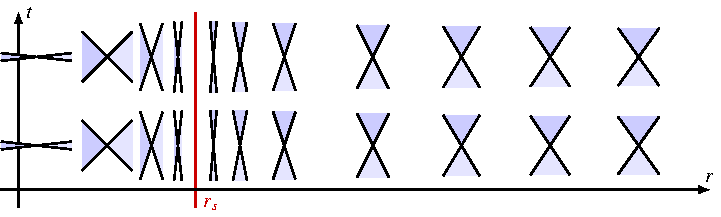
\includegraphics{chapters/110-kruemmung/images/sl.pdf}
\caption{Entstehung des Ereignishorizontes bei einem schwarzen Loch.
Ausser von $r=r_s$ 
Innerhalb $r=r_s$ ist die Richtung der Zukunft ausschliesslich zu
abnehmenden Werten von $r$ gerichtet.
Teilchen können sich also nur noch auf Bahnen bewegen, die innerhalb
$r_S$ bleiben.
\label{buch:kruemmung:schwarzesloch:fig:sl}}
\end{figure}

%
In einem $r$-$ct$-Diagramm entspricht das zwei Linien, die
in einem Winkel 
\[
\alpha = \arctan \biggl(1-\frac{r_s}{r}\biggr)
\]
zur $r$-Achse stehen.
Die beiden Richtungen sind in
Abbildung~\ref{buch:kruemmung:schwarzesloch:fig:sl}
durch schwarze Linien angezeigt.

Der Bereich der Zukunft oder Verangenheit von einem Weltpunkt aus
wird durch negative Werte der Metrik angezeigt.
Für $r>r_s$ ist dies der Bereich zwischen den beiden Strahlen in
$t$-Richtung.
Für $r<r_s$ kehrt jedoch das Vorzeichen der Metrik, der Kegel der
Zukunft zeigt jetzt in Richtung abnehmender $r$.
In Abbildung~\ref{buch:kruemmung:schwarzesloch:fig:sl} ist die
Zukunft durch ein blaues Dreieck angezeigt, die Vergangenheit durch
helleres Blau.
Dies bedeutet, dass ein Teilchen nach dem Überschreiten der Grenze $r=r_s$
sich nur noch in Richtung abnehmender $r$ bewegen kann, die Zukunft des
Teilchens befindet sich vollständig innerhalb $r_s$.

Aus dem Bereich $r_s$ gibt es also kein Entkommen, nicht einmal
für Lichtstrahlen.
Man sagt, bei $r_s$ befinde sich der \emph{Ereignishorizont}.
\index{Ereignishorizont}%
Ein Objekt mit einem Radius, der kleiner ist als sein Schwarzschild-Radius
wird daher als \emph{schwarzes Loch} bezeichnet.
\index{schwarzes Loch}%
Von aussen gibt es keine Möglichkeit, irgend etwas darüber zu sagen,
was innerhalb des Schwarzschild-Radius passiert.

%
% Rotierende Objekte und die Kerr-Metrik
%
\subsection{Rotierende Objekte und die Kerr-Metrik}
Übliche Modelle der Sternentstehung zeigen allerdings, dass es fast
unmöglich ist, dass ein Objekt von der Grösse eines Sterns keinen 
verbleibenden Drehimpuls hat.
Noch dramatischer wird die Situation bei Neutronensternen, wo 
Rotationsfrequenzen von bis zu $716\,\text{Hz}$ gemessen worden sind.
Da Neutronensterne auch sehr hohe Masse bei kleinen Abmessungen
aufweisen, kann nur die allgemeine Relativitätstheorie das Gravitationsfeld
adäquat beschreiben.
Eine Lösung ist die von Roy Kerr gefundene \emph{Kerr-Metrik},
die aber hier nicht weiter diskutiert wird.
\index{Kerr, Roy}%
\index{Kerr-Metrik}%


%
% Die Friedmann-Gleichung und die Geschichte des Universums
%
\section{Die Friedmann-Gleichungen und die Geschichte des Universums
\label{buch:kruemmung:section:friedmann}}
\kopfrechts{Die Friedmann-Gleichungen}%
Vor dem frühen 20.~Jahrhundert gab es weder theoretische noch experimentelle
Hinweise darauf, dass das Universum sich über die Zeit verändern könnte.
Es wurde daher allgemein angenommen, dass das Universum immer gleich
ausgesehen hat.
Es gab daher auch keine Möglichkeit und keinen Bedarf, eine Theorie der
Geschichte des Universums zu entwickeln.
Die allgemeine Relativitätstheorie ermöglichte erstmals, das ganze
Universum mathematisch zu erfassen und damit seine Geschichte aus
den aktuellen Beobachtungen zu extrapolieren.

1923 konnte Edwin Hubble nachweisen, dass der Andromeda-Nebel, wie
\index{Hubble, Edwin}%
er damals genannt wurde, eine eigene Galaxie weit ausserhalb unserer
eigenen ist.
Dazu verwendete er den Zusammenhang zwischen absoluter Helligkeit
und Periode gewisser veränderlicher Sterne, die er auch in der
Andromeda-Galaxie fand.
\index{Andromeda-Galaxie}%
Die Methode ermöglicht erstmals, die Distanzmessung bis zu nahen Galaxien
zu erstrecken.
Messungen von Galaxienspektren durch Milton Humason 
\index{Humason, Milton}%
zeigte eine Rotverschiebung, entfernte Galaxien scheinen sich zu
\index{Rotverschiebung}%
entfernen.
1929 postulierte Hubble aufgrund weiterer Messungen einen linearen
Zusammenhang zwischen Rotverschiebung und Entfernung, die heute
das hubblesche Gesetz genannt wird.
\index{hubblesches Gesetz}%
\index{Gesetz!von Hubble}%
Sie liess den Schluss zu, dass sich das ganze Universum ausdehnt.
Aus der Ausdehnungsgeschwindigkeit, der sogenannten 
\emph{Hubble-Konstante} $H_0$
\index{Hubble-Konstante}%
lässt sich auch erstmals eine Schätzung für das Alter des Universums
abgeben.

%
% Das kosmologische Prinzip
%
\subsection{Das kosmologische Prinzip}
Die einsteinschen Feldgleichungen beschreiben die Metrik in Abhängigkeit
von der Verteilung von Energie und Impuls im Universum.
Doch wie soll man diese messen?
Über kleine Distanzen zum Beispiel innerhalb unserer Galaxie ist die
Massedichte extrem unterschiedlich:
Neutronensterne haben extrem hohe Dichte, aber der grösste Teil des
Universums ist ein sehr gutes Vakuum.
Aber auch noch über die Distanzen zwischen Galaxien gibt es grosse
Unterschiede: Materie im Universum scheint vor allem in Galaxien
zusammengeklumpt zu sein, dazwischen findet man fast nichts.
Über noch grössere Distanzen scheinen auch die Galaxien in Clustern
mit grossen leeren Räumen genannt ``voids'' dazwischen organisiert
zu sein.

Andererseits gibt es keinen Grund, dass die Erde mit ihrer Sonne, ihrer
eigenen Milchstrasse und den wenigen Galaxien der lokalen Gruppe in
irgend einer Form speziell sein sollte.
Daraus lässt sich das \emph{kosmologische Prinzip} ableiten.
\index{kosmologisches Prinzip}%
Es besagt, dass das Universum homogen und isotrop ist.
\emph{Homogen} bedeutet, dass an jedem Punkt die gleichen Verhältnisse
anzutreffen sind.
\index{homogen}%
\emph{Isotrop} bedeutet, dass keine Richtung im Universum speziell ist.
Im Grossen ist daher das Universum gefüllt mit einem Gas konstanter
Dichte.
\index{isotrop}%
Die rechte Seite der einsteinschen Feldgleichungen ist für die 
Zwecke der relativistischen Kosmologie ein räumlich konstanter Tensor.

%
% Die Robertson-Walker-Metrik
%
\subsection{Die Friedmann-Lema\^\i tre-Robertson-Walker-Metrik}
Auch die Lösung der einsteinschen Feldgleichungen muss die vom
kosmologischen Prinzip geforderten Eigenschaften erfüllen.
Die Metrik und die zugehörige Krümmung darf nicht vom Ort
abhängen.
Nur eine Zeitabhängigkeit darf übrig bleiben, die mit hubbleschen
Gesetz der Ausdehnung des Universums kompatibel sein muss.

Die homogenen und isotropen Räume können mit den Methoden der
riemannschen Geometrie untersucht und klassifiziert werden.
Man kann zeigen, dass dreidimensionale Räume konstanter Krümmung 
die Metrik
\[
ds^2
=
\frac{dr^2}{1-kr^2} + r^2\,(d\vartheta^2 + \sin\vartheta\,d\varphi^2)
\]
haben, wobei $k$ der sogenannte \emph{Krümmungsparameter} ist.
Für $k=0$ entsteht die bekannte euklidische Metrik.

Die Beobachtungen von Hubble zeigen, dass Distanzen zwischen
den Galaxien mit der Zeit grösser werden.
Diese Zeitabhängigkeit kann mit einer Funktion $a(t)$ beschrieben
werden, die zum heutigen Zeitpunkt $t_0$ den Wert $a(t_0)=1$ hat.
Die Metrik
\begin{equation}
ds^2
=
a(t)^2
\biggl(
\frac{dr^2}{1-kr^2} + r^2\,(d\vartheta^2 + \sin\vartheta\,d\varphi^2)
\biggr)
\label{buch:kruemmung:kosmologie:eqn:ads}
\end{equation}
beschreibt Abstände, die um den Faktor $a(t)$ grösser werden.

Die Zeitabhängigkeit muss zu jedem Zeitpunkt eine Minkowski-Metrik
ergeben, damit im Grenzfall ohne Gravitation die empirisch bestätigte
spezielle Raum-Zeit-Struktur des Universums entsteht.
Es resultiert die Metrik der folgenden Definition.

\begin{definition}[Friedmann-Lema\^\i tre-Robertson-Walker-Metrik]
Die \emph{Friedmann-Le\-ma\^\i tre-Robertson-Walker-Metrik} ist die Metrik
\index{Friedmann-Lemaitre-Robertson-Walker-Metrik@Friedmann-Lema\^\i tre-Robertson-Walker-Metrik}%
mit dem Linienelement
\begin{equation}
ds^2
=
c^2\,dt^2
-
a(t)^2\biggl(
\frac{dr^2}{1-kr^2} + r^2\,(d\vartheta^2 + \sin\vartheta\,d\varphi^2)
\biggr)
\end{equation}
Die Funktion $a(t)$ heisst der Skalenfaktor und hat den Wert $a(t_0)=1$
zum aktuellen Zeitpunkt $t_0$.
\index{Skalenfaktor}%
\end{definition}

Um die Geschichte des Universums zu ergründen müssen also sowohl der
Krümmungsparameter $k$ wie auch die Funktion $a(t)$ bestimmt werden.
Aus dem hubbleschen Gesetz ist ausserdem bekannt, wie schnell $a(t)$
ändert, es ist $\dot{a}(t)=H_0$.
Es würde also genügen, eine Differentialgleichung zweiter Ordnung
für $a(t)$ zu finden.
Eine solche müsste sich aus den einsteinschen Feldgleichungen 
gewinnen lassen.
Dazu sind die Ricci-Krümmung und der Krümmungsskalar zu bestimmen,
was eine ziemlich aufwendige Rechnung ist.
Wir notieren daher hier nur die Resultate.
Die Komponenten des Ricci-Tensors sind
\begin{align*}
R_{00}
&=
-3 \frac{\ddot{a}(t)}{a(t)}
\\
R_{ik}
&=
-
\biggl(
\frac{\ddot{a}(t)}{a(t)} + 2\frac{\dot{a}(t)^2}{a(t)^2}+\frac{2k}{a(t)^2}
\biggr)
g_{ik},
\intertext{der Krümmungsskalar wird}
R
&=
-6
\biggl(
\frac{\ddot{a}(t)}{a(t)} + \frac{\dot{a}(t)^2}{a(t)^2}+\frac{k}{a(t)^2}
\biggr).
\end{align*}
Die Komponenten des Einstein-Tensors können daraus wie folgt
ermittelt werden:
\begin{equation}
G_{\mu\nu}
=
R_{\mu\nu} - \frac12 g_{\mu\nu} R
\qquad\Rightarrow\qquad
\left\{
\begin{aligned}
G_{00}
&=
\frac{3}{2}
\frac{\dot{a}(t)^2}{a(t)^2} 
+\frac{k}{a(t)^2}
\\
G_{ii}
&=
2
\frac{\ddot{a}(t)}{a(t)}
+
\frac{\dot{a}(t)^2}{a(t)}
+
\frac{k}{a(t)^2}.
\end{aligned}
\right.
\label{buch:kruemmung:kosmologie:eqn:G}
\end{equation}

%
% Die Friedmann-Gleichung
%
\subsection{Die Friedmann-Gleichung}
Mit Hilfe des Einstein-Tensors, der in \eqref{buch:kruemmung:kosmologie:eqn:G}
berechnet wurde, kann man jetzt auch die Einstein-Gleichungen
für das Universum aufstellen.
Dazu braucht man aber auf der rechten Seite der Gleichung einen 
Ausdruck für den Energie-Impuls-Tensor.
Seine $00$-Komponente enthält die Massedichte, die anderen diagonalen
Komponenten geben die Energie wieder, die von der Bewegung der
Teilchen herrührt.
Sie äussert sich im Druck $p$ des Gases.
Die Komponenten von $T_{ik}$ sind daher
\begin{equation}
\begin{aligned}
T_{00} &= c^2 \varrho 
\\
T_{ii} &= -p g_{ii}&&\text{für $i>0$}
\end{aligned}
\end{equation}
Einsetzen in die einsteinsche Feldgleichung
\eqref{buch:kruemmung:feldgleichung:eqn:feldgleichung}
folgen die Gleichungen
\begin{align*}
6
\frac{\dot{a}(t)^2}{a(t)^2} 
+\frac{k}{a(t)^2}
&=
\frac{8\pi G}{c^4}c^2\varrho
&&\Rightarrow&
\biggl(\frac{\dot{a}(t)}{a(t)}\biggr)^2
+
\frac{k}{a(t)^2}
&=\frac{4\pi G\varrho}{c^2}
\\
2
\frac{\ddot{a}(t)}{a(t)}
+
\frac{\dot{a}(t)^2}{a(t)}
+
\frac{k}{a(t)^2}
&=
-\frac{8\pi G}{c^4}p.
\end{align*}
Diese beiden Gleichungen heissen auch die 
\emph{Friedmann-Gleichungen}.
\index{Friedmann-Gleichungen}
Sie wurden von Aleksander Friedmann 1922 hergeleitet.
Sie beschreiben, wie der Skalenfaktor $a(t)$ des Universums sich
mit der Zeit verändern kann.

Zur vollständigen Lösung der Friedmann-Gleichungen braucht man 
zusätzliche Information über die Abhängigkeit von $\varrho$
und $p$ vom Skalenfaktor.
\begin{itemize}
\item
Ein gewöhnliches Gas wird die Dichte mit zunehmendem Skalenfaktor
wie $a(t)^{-3}$ abnehmen.
\item
Für die im Universum vorhandene Strahlung gilt dies jedoch nicht.
Bei der Ausdehnung wird die Wellenlänge der Strahlung ebenfalls um
den Faktor $a(t)$ gestreckt, die Energie eines Photons wird daher
um den Faktor $a(t)^{-1}$ geringer.
Zusammen mit der Abnahme der Dichte der Photonen wird der
Strahlungsdruck daher wie $a(t)^{-4}$ abnehmen.
\item
In den letzten Jahrzehnten hat sich gezeigt, dass die beobachtbare
Materie (inklusive der dunklen Materie) und Strahlung nicht ausreicht,
um das verhalten des Universums zu erklären.
Die sogenannte \emph{dunkle Energie} füllt das Vakuum gleichmässig
aus.
Insbesondere hängt sie nicht von $a(t)$ ab.
\index{dunkle Energie}%
\end{itemize}
Die Entwicklung des Radius des Universums hängt also auch vom Energiemix
des Universums ab.

%
% Ds Alter des Universums
%
\subsection{Das Alter des Universums}
Kennt man die Anteile der verschiedenen Komponenten im
Energie-Impuls-Tensor, kann man aus den Friedmann-Gleichungen eine
Formel für das Alter des Universums herleiten.
Für
\begin{itemize}
\item
$\Omega_r$: Anteil der Strahlung an der Energiedichte im heutigen
Universum.
Das heutige Universum ist sehr dunkel, der Strahlungsanteil ist
nur etwa $5.5\cdot10^{-5}$.
\item
$\Omega_m$: Anteil der Materie (inklusive dunkler Materie) an der
Energiedichte im heutigen Universum.
\item
$\Omega_k$: Beitrag des Krümmungsparameters.
Beobachtungen der Inhomogeneitäten des kosmischen Mikrowellenhintergrundes
haben gezeigt, dass dieser Beitrag sehr klein ist.
\item
$\Omega_\Lambda$: Anteil der dunklen Energie an der Energiedichte im 
heutigen Universum.
Nach aktuellem Wissen macht die dunkle Energie mehr als zwei Drittel
der Energiedichte aus.
\end{itemize}
lautet die Formel
\begin{equation}
t_0
=
\frac{1}{H_0}
\int_0^{a_0}
\frac{da}{\!\sqrt{\Omega/a^2 + \Omega_m/a + \Omega_k + \Omega_\Lambda a^2}}.
\label{buch:kruemmung:kosmologie:eqn:alter}
\end{equation}
Die Exponenten des Skalenfaktors reflektieren die Abhängigkeit 
der Energiedichte der entsprechenden Komponente vom den Skalenfaktor.

Mit der Formel
\eqref{buch:kruemmung:kosmologie:eqn:alter}
kann man für die experimentell von der Planck-Mission bestimmten Werte
\begin{align*}
H_0 &= 67.15\,\textrm{km/s/Mpc} &
\Omega_m &= 0.315,&
\Omega_r &= 5.5\cdot 10^{-5},&
\Omega_\Lambda &= 0.685,&
\Omega_k &< 0.005
\end{align*}
das Alter von $13.844\,\textrm{Gyr}$ finden.

%



